\documentclass[a4paper,final]{article}
\usepackage[14pt]{extsizes}
\usepackage[T2A]{fontenc}
\usepackage[utf8]{inputenc}
\usepackage[russian]{babel}
\usepackage{amsmath}
\usepackage[left=20mm, top=20mm, right=20mm, bottom=20mm, footskip=10mm]{geometry}
\usepackage{ragged2e}
\usepackage{setspace}
\usepackage{alltt}
\usepackage{wrapfig}
\usepackage{moreverb} %листинги
\usepackage{indentfirst} % для абзацного отступа
\renewcommand\verbatimtabsize{4\relax}
\renewcommand\listingoffset{0.2em} %отступ от номеров строк
\renewcommand{\arraystretch}{1.4} % высота строки
\usepackage[font=small, singlelinecheck=false, justification=raggedleft, format=plain, labelsep=period]{caption} %заголовок таблицы
\usepackage{listings}
\usepackage{xcolor} % цвета
\usepackage{hyperref}% для гиперссылок
\usepackage{enumitem} %для перечислений
\usepackage{nccmath}
\usepackage{tikz}
\usepackage{wrapfig}
\usepackage{listings}
\usepackage{float}
\usepackage{shadow}
\usepackage{longtable}
\usepackage{multirow}
\usepackage{makecell}
\usepackage{longtable}
\usepackage{tabularx}
\usepackage{seqsplit}
\usepackage{subcaption} % Для подрисунков

\hypersetup{colorlinks,
  allcolors=[RGB]{000 000 000}} %гиперссылки

\textheight=24cm
\textwidth=16cm
\oddsidemargin=0pt
\topmargin=-1.5cm
\parindent=24pt % отступ абзаца по горизонтали
\parskip=5pt % отступ абзаца по вертикали
\tolerance=2000 % терпимость
\flushbottom % выравнивание высоты
\addto\captionsrussian{\def\refname{Список использованной литературы}}
\usepackage{xcolor}

%New colors defined below
\definecolor{codegreen}{rgb}{0,0.6,0}
\definecolor{codegray}{rgb}{0.5,0.5,0.5}
\definecolor{codepurple}{rgb}{0.58,0,0.82}
\definecolor{backcolour}{rgb}{0.95,0.95,0.92}


\definecolor{apricot}{HTML}{FFF0DA}
\definecolor{mygreen}{rgb}{0,0.6,0}
\definecolor{string}{HTML}{B40000} % цвет строк в коде
\definecolor{comment}{HTML}{008000} % цвет комментариев в коде
\definecolor{keyword}{HTML}{1A00FF} % цвет ключевых слов в коде
\definecolor{morecomment}{HTML}{8000FF} % цвет include и других элементов в коде
\definecolor{captiontext}{HTML}{FFFFFF} % цвет текста заголовка в коде
\definecolor{captionbk}{HTML}{999999} % цвет фона заголовка в коде
\definecolor{bk}{HTML}{FFFFFF} % цвет фона в коде
\definecolor{frame}{HTML}{999999} % цвет рамки в коде
\definecolor{brackets}{HTML}{B40000} % цвет скобок в коде

\setlist[enumerate,itemize]{leftmargin=1.2cm}

% подгружаемые языки — подробнее в документации listings
\lstloadlanguages{C++}

\newcommand{\doublecline}[1]{\noalign{\vskip-0.5\arrayrulewidth}\cline{#1}\noalign{\vskip-0.5\arrayrulewidth}\cline{#1}}

\begin{document}
\lstset{
  language=C++, % Язык кода по умолчанию
  morekeywords={*,...}, % если хотите добавить ключевые слова, то добавляйте
  % Цвета
  keywordstyle=\color{keyword}\ttfamily\bfseries,
  %stringstyle=\color{string}\ttfamily,
  stringstyle=\ttfamily\color{red!50!brown},
  commentstyle=\color{comment}\ttfamily,
  morecomment=[l][\color{morecomment}]{\#},
  % Настройки отображения
  breaklines=true, % Перенос длинных строк
  basicstyle=\ttfamily\footnotesize, % Шрифт для отображения кода
  backgroundcolor=\color{bk}, % Цвет фона кода
  frame=lrb,xleftmargin=\fboxsep,xrightmargin=-\fboxsep, % Рамка, подогнанная к заголовку
  rulecolor=\color{frame}, % Цвет рамки
  tabsize=3, % Размер табуляции в пробелах
  % Настройка отображения номеров строк. Если не нужно, то удалите весь блок
  numbers=left, % Слева отображаются номера строк
  stepnumber=1, % Каждую строку нумеровать
  numbersep=5pt, % Отступ от кода
  numberstyle=\small\color{black}, % Стиль написания номеров строк
  % Для отображения русского языка
  extendedchars=true,
  literate={Ö}{ {\"O} }1
  {~}{ {\textasciitilde} }1
  {а}{ {\selectfont\char224} }1
  {б}{ {\selectfont\char225} }1
  {в}{ {\selectfont\char226} }1
  {г}{ {\selectfont\char227} }1
  {д}{ {\selectfont\char228} }1
  {е}{ {\selectfont\char229} }1
  {ё}{ {\"e} }1
  {ж}{ {\selectfont\char230} }1
  {з}{ {\selectfont\char231} }1
  {и}{ {\selectfont\char232} }1
  {й}{ {\selectfont\char233} }1
  {к}{ {\selectfont\char234} }1
  {л}{ {\selectfont\char235} }1
  {м}{ {\selectfont\char236} }1
  {н}{ {\selectfont\char237} }1
  {о}{ {\selectfont\char238} }1
  {п}{ {\selectfont\char239} }1
  {р}{ {\selectfont\char240} }1
  {с}{ {\selectfont\char241} }1
  {т}{ {\selectfont\char242} }1
  {у}{ {\selectfont\char243} }1
  {ф}{ {\selectfont\char244} }1
  {х}{ {\selectfont\char245} }1
  {ц}{ {\selectfont\char246} }1
  {ч}{ {\selectfont\char247} }1
  {ш}{ {\selectfont\char248} }1
  {щ}{ {\selectfont\char249} }1
  {ъ}{ {\selectfont\char250} }1
  {ы}{ {\selectfont\char251} }1
  {ь}{ {\selectfont\char252} }1
  {э}{ {\selectfont\char253} }1
  {ю}{ {\selectfont\char254} }1
  {я}{ {\selectfont\char255} }1
  {А}{ {\selectfont\char192} }1
  {Б}{ {\selectfont\char193} }1
  {В}{ {\selectfont\char194} }1
  {Г}{ {\selectfont\char195} }1
  {Д}{ {\selectfont\char196} }1
  {Е}{ {\selectfont\char197} }1
  {Ё}{ {\"E} }1
  {Ж}{ {\selectfont\char198} }1
  {З}{ {\selectfont\char199} }1
  {И}{ {\selectfont\char200} }1
  {Й}{ {\selectfont\char201} }1
  {К}{ {\selectfont\char202} }1
  {Л}{ {\selectfont\char203} }1
  {М}{ {\selectfont\char204} }1
  {Н}{ {\selectfont\char205} }1
  {О}{ {\selectfont\char206} }1
  {П}{ {\selectfont\char207} }1
  {Р}{ {\selectfont\char208} }1
  {С}{ {\selectfont\char209} }1
  {Т}{ {\selectfont\char210} }1
  {У}{ {\selectfont\char211} }1
  {Ф}{ {\selectfont\char212} }1
  {Х}{ {\selectfont\char213} }1
  {Ц}{ {\selectfont\char214} }1
  {Ч}{ {\selectfont\char215} }1
  {Ш}{ {\selectfont\char216} }1
  {Щ}{ {\selectfont\char217} }1
  {Ъ}{ {\selectfont\char218} }1
  {Ы}{ {\selectfont\char219} }1
  {Ь}{ {\selectfont\char220} }1
  {Э}{ {\selectfont\char221} }1
  {Ю}{ {\selectfont\char222} }1
  {Я}{ {\selectfont\char223} }1
  {\{}{ { {\color{brackets}\{} } }1 % Цвет скобок {
  {\} }{ { {\color{brackets}\} } } }1 % Цвет скобок }
}


\thispagestyle{empty}
\begin{center}
\hfill \break
\hfill \break
\normalsize{МИНИСТЕРСТВО НАУКИ И ВЫСШЕГО ОБРАЗОВАНИЯ РОССИЙСКОЙ ФЕДЕРАЦИИ\\
 федеральное государственное автономное образовательное учреждение высшего образования «Санкт-Петербургский политехнический университет Петра Великого»\\[10pt]}
\normalsize{Институт компьютерных наук и кибербезопасности}\\[10pt] 
\normalsize{Высшая школа технологий искусственного интеллекта}\\[10pt] 
\normalsize{Направление: 02.03.01 <<Математика и компьютерные науки>>}\\
\vspace{50pt}
{\large Математическая логика и теория формальных языков\\
Отчёт о выполнении лабораторной работы №1 \\
<<Проверка корректности модели автомобиля марки ВАЗ, УАЗ, ГАЗ и Москвич через реализацию конечного автомата для регулярного выражения>>\\[1em]
Вариант 35}
\end{center}
 \vspace{70pt}
\small{ 
\begin{tabular}{lrrl}
\!\!\!Студент, & \hspace{2cm} & & \\
\!\!\!группа 5130201/30102 & \hspace{2cm} & \underline{\hspace{3cm}} & Путята М. А.  \\\\
\!\!\!Преподаватель & \hspace{2cm} & \underline{\hspace{3cm}} &  Востров А. В. \\\\
&&\hspace{5cm}
\end{tabular}
\begin{flushright}
<<\underline{\hspace{1cm}}>>\underline{\hspace{2.5cm}} 2026 г.
\end{flushright}
}

\hfill \break
\begin{center} \small{Санкт-Петербург, 2026} \end{center}


\newpage
\tableofcontents
\newpage

\section*{Введение}
\addcontentsline{toc}{section}{Введение}

Целью данной работы является разработка программы, которая сможет определять корректность введённых пользователем строк и генерировать новые корректные строки, используя детерминированный конечный автомат.

\textbf{Задание}: По заданному варианту построить регулярное выражение, затем недетерминированный конечный автомат и детерминировать его (переходы можно задавать диапазонами). Реализовать программу, которая проверяет введенный текст через реализацию конечного автомата (варианты вывода: строка соответствует, не соответствует, символы не из алфавита). Также необходимо реализовать функцию случайной генерации верной строки по полученному конечному автомату.

\textbf{Вариант 35}: Проверка правильно введенной марки автомобиля ВАЗ, УАЗ, ГАЗ, Москвич (с учетом старых моделей).

Для выполнения поставленной задачи необходимо:
\begin{enumerate}
    \item Построить регулярное выражение, соответствующее варианту.
    \item По полученному регулярному выражению построить недетерминированный конечный автомат.
    \item Детерминировать конечный автомат.
    \item Создать программную реализацию конечного автомата.
    \item Создать инструменты для проверки корректности строк и генерации корректных строк.
\end{enumerate}

\newpage
\section{Математическое описание}
\subsection{Регулярное выражение}
\textbf{Регулярное выражение} -- способ описания регулярных языков над конечным словарём $\Sigma$.

Регулярное выражение состоит из:
\begin{itemize}
    \item базовых элементов:
    \begin{itemize}
        \item $\emptyset$ -- пустое множество символов;
        \item $\epsilon$ -- пустая цепочка символов;
        \item $a \in \Sigma$ -- любой символ из словаря $\Sigma$;
    \end{itemize}
    \item операций:
    \begin{itemize}
        \item \textbf{Конкатенация} $R_1R_2$ -- множество цепочек, образованных соединением цепочек $R_1$ и $R_2$.
        \item \textbf{Объединение} $R_1 + R_2$ или $R_1 | R_2$ -- множество цепочек, принадлежащих $R_1$ или $R_2$.
        \item \textbf{Итерация Клини} $R^*$ -- множество цепочек, состоящих из нуля и более повторений цепочки R.
        \item \textbf{Усеченная итерация} $R^+$ -- множество цепочек, состоящих из 1 и более повторений цепочки R.
    \end{itemize}
\end{itemize}

Приоритеты операций:
\begin{enumerate}
    \item Итерация Клини.
    \item Усечённая итерация.
    \item Конкатенация.
    \item Объединение.
\end{enumerate}

Для изменение порядка выполнения операций можно использовать круглые скобки <<(>> и <<)>>.


\textbf{Регулярное множество} -- это бесконечное множество цепочек построенных, построенных из символов конечного словаря с использованием вышеперечисленных операций.

Например, регулярное выражение <<$a^*b + cd^+$>> будет задавать следующее множество:$$\{b, ab, aab, aaab, ...\} \cup \{ cd, cdd, cddd, ... \}$$

\textbf{Регулярный язык} -- подмножество $\Sigma^*$, которое можно описать с помощью регулярного выражения.

\textbf{Операции над регулярными языками}

Пусть $L_1 \text{ и } L_2 \subseteq \Sigma^*$, тогда для данных языков определены следующие операции.

\begin{itemize}
    \item \textbf{Конкатенация}: $L_1 \cdot L_2 = \{ w_1w_2 ~|~ w_1 \in L_1 \wedge w_2 \in L_2 \}$.

    Пример: $\{ a, b \} \cdot \{ b, c \} = \{ ab, ac, bb, bc\}$
    \item \textbf{Объединение}: $L_1 \cup L_2 = \{ w ~|~ w \in L_1 \vee w \in L_2 \}$.

    Пример: $\{ a, b \} \cup \{ b, c \} = \{ a, b, c \}$
    \item \textbf{Итерация Клини}: $L^* = \bigcup_{k=0}^\infty L^k$, где $L^{k+1} = L^k \cdot L$, $L^0 = \{ \epsilon \}$.

    Пример: $\{a, b\}^* = \{\epsilon, a, aa, ab, baaaba, ...\}$
    \item \textbf{Усечённая итерация}: $L^* = \bigcup_{k=1}^\infty L^k$

    Пример: $\{a, b\}^* = \{a, aa, ab, baaaba, ...\}$
\end{itemize}

Регулярные языки, реализуемые через регулярные выражения, лежат в основе обработки текстовой информации, поиска шаблонов, валидации данных и лексического анализа.

\subsection{Регулярное выражение используемое в работе}
Для определения корректности введённой модели автомобиля было создано 4 регулярных выражения для каждой рассматриваемой марки автомобиля:
\begin{itemize}
    \item регулярное выражения для моделей автомобилей марки ГАЗ:\\[0.7em]
    <<ГАЗ (1[2348]|2([1245]|(3(08|30)))|31(0(2(21?|9)?|[35])|1(05?|1))|46|6[1479]|А|М-(1|20|72)\\|Siber)>>
    \item регулярное выражение для моделей автомобилей марки УАЗ:\\[0.7em]
    <<УАЗ (2(206|3(15|6(08|[25]|32))|7(46|60|722)|9232)|3(1(5(0|1[249]?|3|9)|6[025])|303|741|9\\(09[45]?|625?))|469|Cargo|Combi|Hunter|Patriot|Pickup|Profi)>>
    \item регулярное выражение для моделей автомобилей марки Москвич:\\[0.7em]
    <<Москвич (21(3[678]|4[012])|3|4(0[0-37-8]|1[012]|2[3467]|3(0|4П))|[568]|Дуэт|Иван \\Калита|Князь Владимир|Святогор|Юрий Долгорукий)>>
    \item регулярное выражение для моделей автомобилей марки ВАЗ:\\[0.7em]
    <<(ВАЗ|LADA) (1111|2(1(0[1-9]|1[0-5]|2[0139]|31)|32[89])|Aura|EL Lada|Granta|Iskra\\|Kalina|Largus|Niva|Priora|Revolution|Vesta|XRAY)>>
    
\end{itemize}

Далее данные регулярные выражение были объединены с помощью трёх операторов <<|>> и было получено итоговое регулярное выражение для всех четырёх марок автомобилей:\\[0.7em]
<<ГАЗ (1[2348]|2([1245]|(3(08|30)))|31(0(2(21?|9)?|[35])|1(05?|1))|46|6[1479]|А|М-(1|20|72)\\|Siber)|УАЗ (2(206|3(15|6(08|[25]|32))|7(46|60|722)|9232)|3(1(5(0|1[249]?|3|9)|6[025])|303|741\\|9(09[45]?|625?))|469|Cargo|Combi|Hunter|Patriot|Pickup|Profi)|Москвич (21(3[678]|4[012])|\\3|4(0[0-37-8]|1[012]|2[3467]|3(0|4П))|[568]|Дуэт|Иван Калита|Князь Владимир|Святогор|\\Юрий Долгорукий)|(ВАЗ|LADA) (1111|2(1(0[1-9]|1[0-5]|2[0139]|31)|32[89])|Aura|EL Lada|\\Granta|Iskra|Kalina|Largus|Niva|Priora|Revolution|Vesta|XRAY)>>

\subsection{Конечный автомат}
Конечный автомат -- математическая модель, определяющаяся набором $A = (S, \Sigma, Y, S0, \delta, \lambda)$, где:
\begin{itemize}
    \item S = \{ S0 \} $\cup$ \{VAZ1, \dots, VAZ3\} $\cup$ \{LADA1, \dots LADA4\} $\cup$ \{ V0, \dots V18 \} $\cup$ \{ MOS1, \dots, MOS20 \} $\cup$ \{ M0, \dots, M20 \} $\cup$ \{ GAZ1, \dots, GAZ3 \} $\cup$ \{ G0, \dots, G33 \} $\cup$ \{ UAZ1, \dots, UAZ3 \} $\cup$ \{ U1, \dots U52 \} -- конечное множество состояний;
    \item $\Sigma$ = \{ ''\_'' , -, 0, 1, 2, 3, 4, 5, 6, 7, 8, 9, A, C, D, E, G, H, I, K, L, M, N, P, R, S, V, X, Y, a, b, c, d, e, f, g, i, k, l, m, n, o, p, r, s, t, u, v, А, В, Г, Д, З, И, К, М, П, С, У, Ю, а, в, г, д, з, и, й, к, л, м, н, о, р, с, т, у, ч, ь, э, я \} -- конечное множество входных сигналов;
    \item $Y = \{  \}$ -- конечное множество выходных сигналов;
    \item $S0$ -- начальное состояние, при этом $S0 \in S$;
    \item $\delta : S \times \Sigma \rightarrow S$ -- функция переходов;
    \item $\lambda: S \times \Sigma \rightarrow Y$ -- функция выходов;
\end{itemize}

Различают недетерминированные (НДКА) и детерминированные конечные автоматы (ДКА). Основным отличием НДКА от ДКА является наличие $\epsilon$-переходов и возможность неоднозначных переходов.

\subsection{Недетерминированный конечный автомат}
Недетерминированные конечные автоматы крайне удобны для создания распознавателей, так как:
\begin{itemize}
    \item обычно имеют меньше состояний, чем детерминированные конечные автоматы;
    \item наличие $\epsilon$-переходов упрощает создание композиций из НДКА;
    \item регулярные выражения легко преобразуются в НДКА.
\end{itemize}

По полученным регулярным выражениям было построено 4 НДКА, каждый из которых соответствует определённой марке автомобиля. Данные НДКА представлены на рисунках 1 - 4.

\begin{figure}[H]
    \centering
    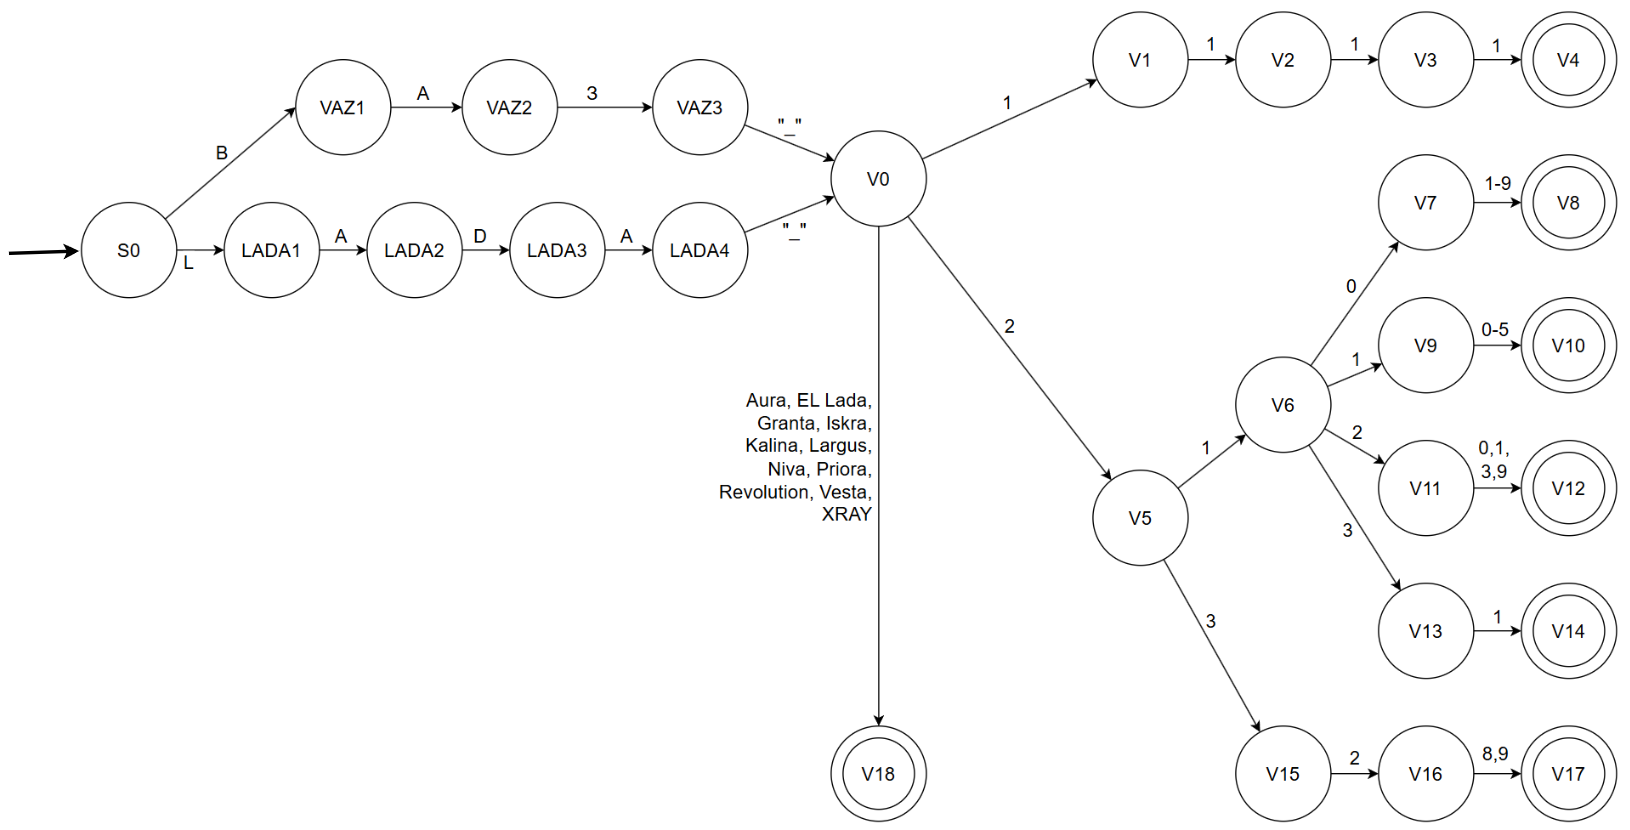
\includegraphics[width=0.75\linewidth]{ndka1.png}
    \caption{\centeringНДКА для ВАЗ}
\end{figure}

\begin{figure}[H]
    \centering
    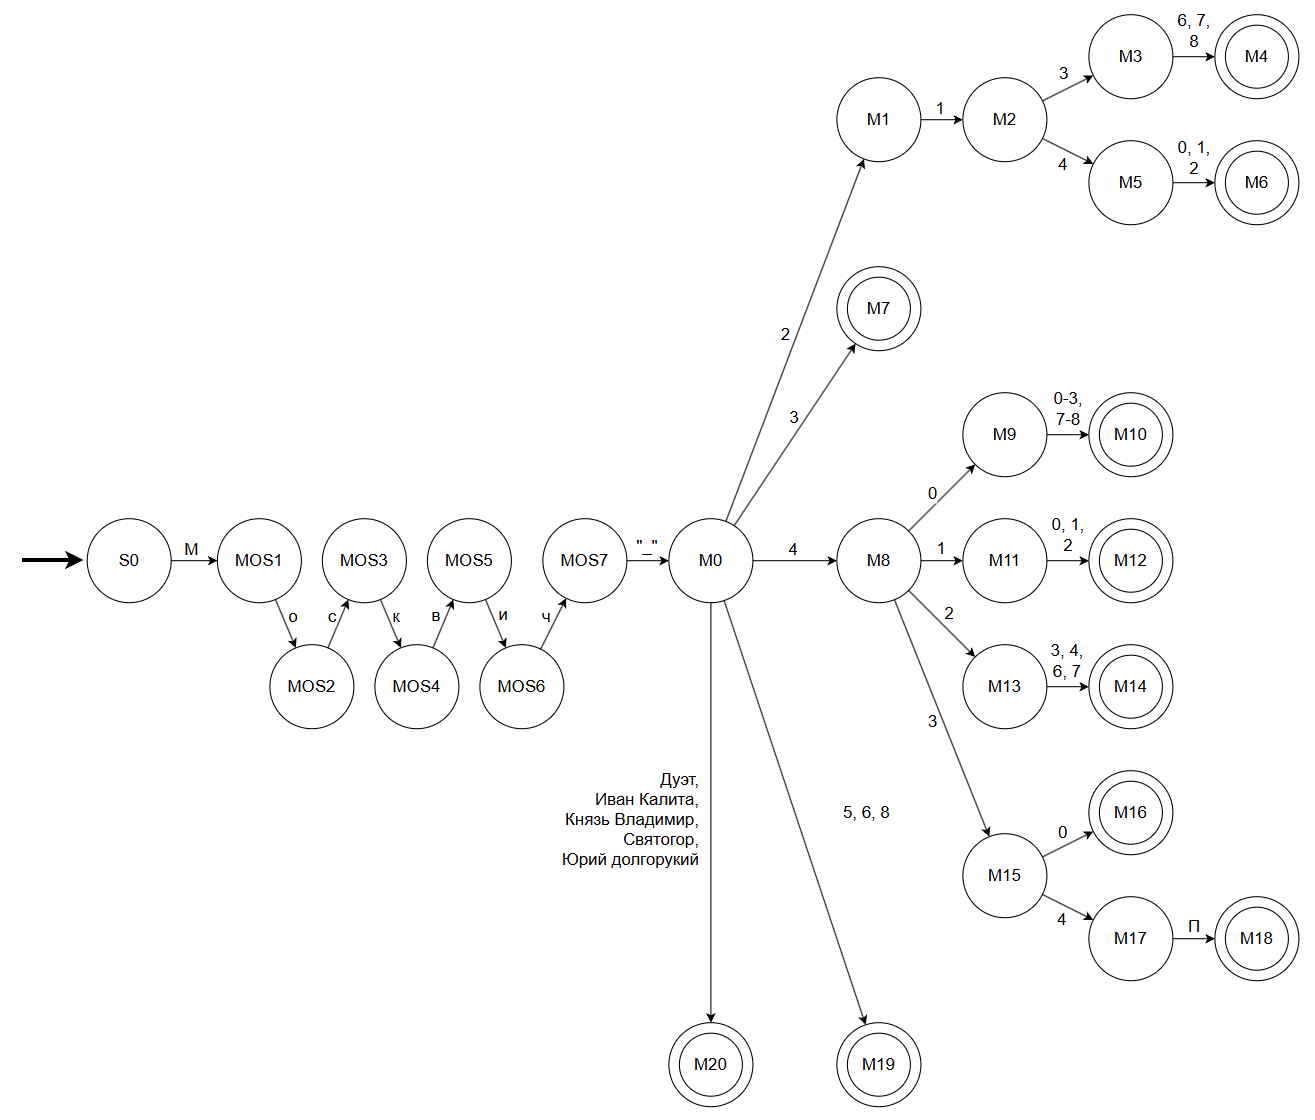
\includegraphics[width=0.6\linewidth]{ndka4.png}
    \caption{\centeringНДКА для Москвич}
\end{figure}

\begin{figure}[H]
    \centering
    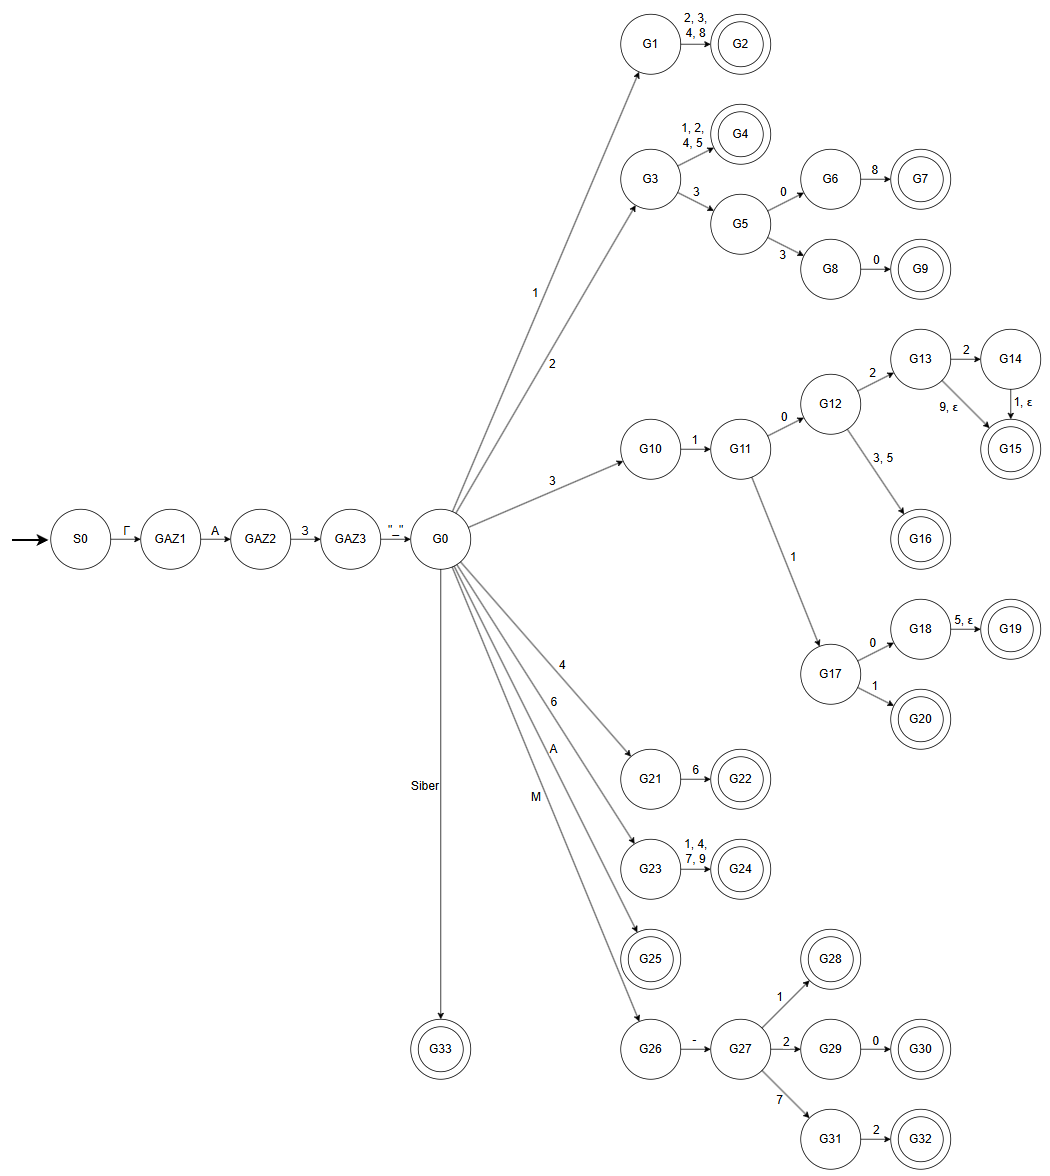
\includegraphics[width=0.65\linewidth]{ndka3.png}
    \caption{\centeringНДКА для ГАЗ}
\end{figure}

\begin{figure}[H]
    \centering
    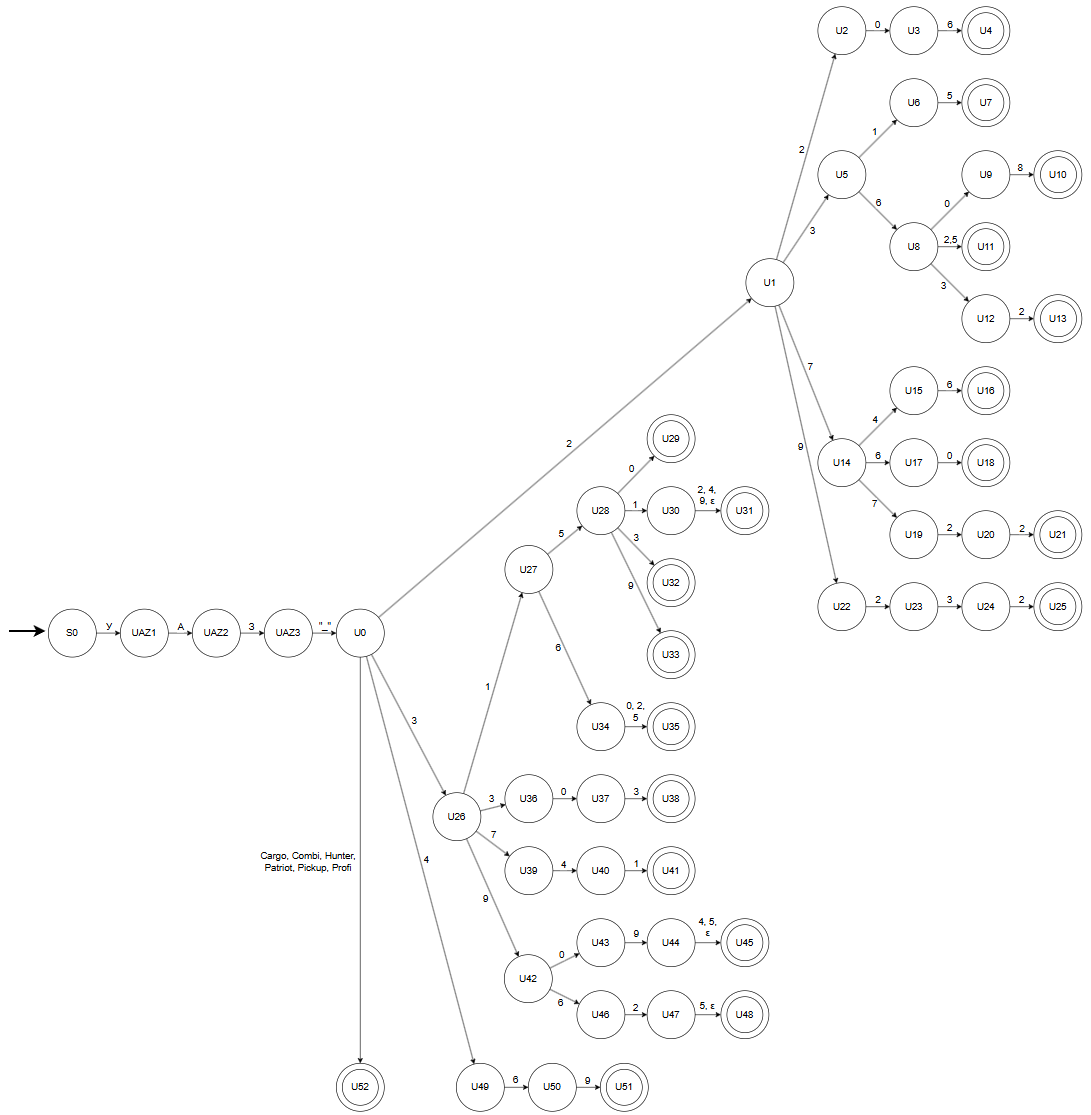
\includegraphics[width=0.75\linewidth]{ndka2.png}
    \caption{\centeringНДКА для УАЗ}
\end{figure}

Далее созданные НДКА были объединены в один НДКА с начальным состоянием $S_0$. Из начального состояния существует 5 переходов, в зависимости от которых выбирается марка, корректность модели автомобиля которой будет проверяться:
\begin{itemize}
    \item <<В>> или <<L>> -- ВАЗ (LADA);
    \item <<У>> -- УАЗ;
    \item <<Г>> -- ГАЗ;
    \item <<М>> -- Москвич.
\end{itemize}

Полученный недетерминированный конечный автомат представлен на рисунке 5.

\begin{figure}[H]
    \centering
    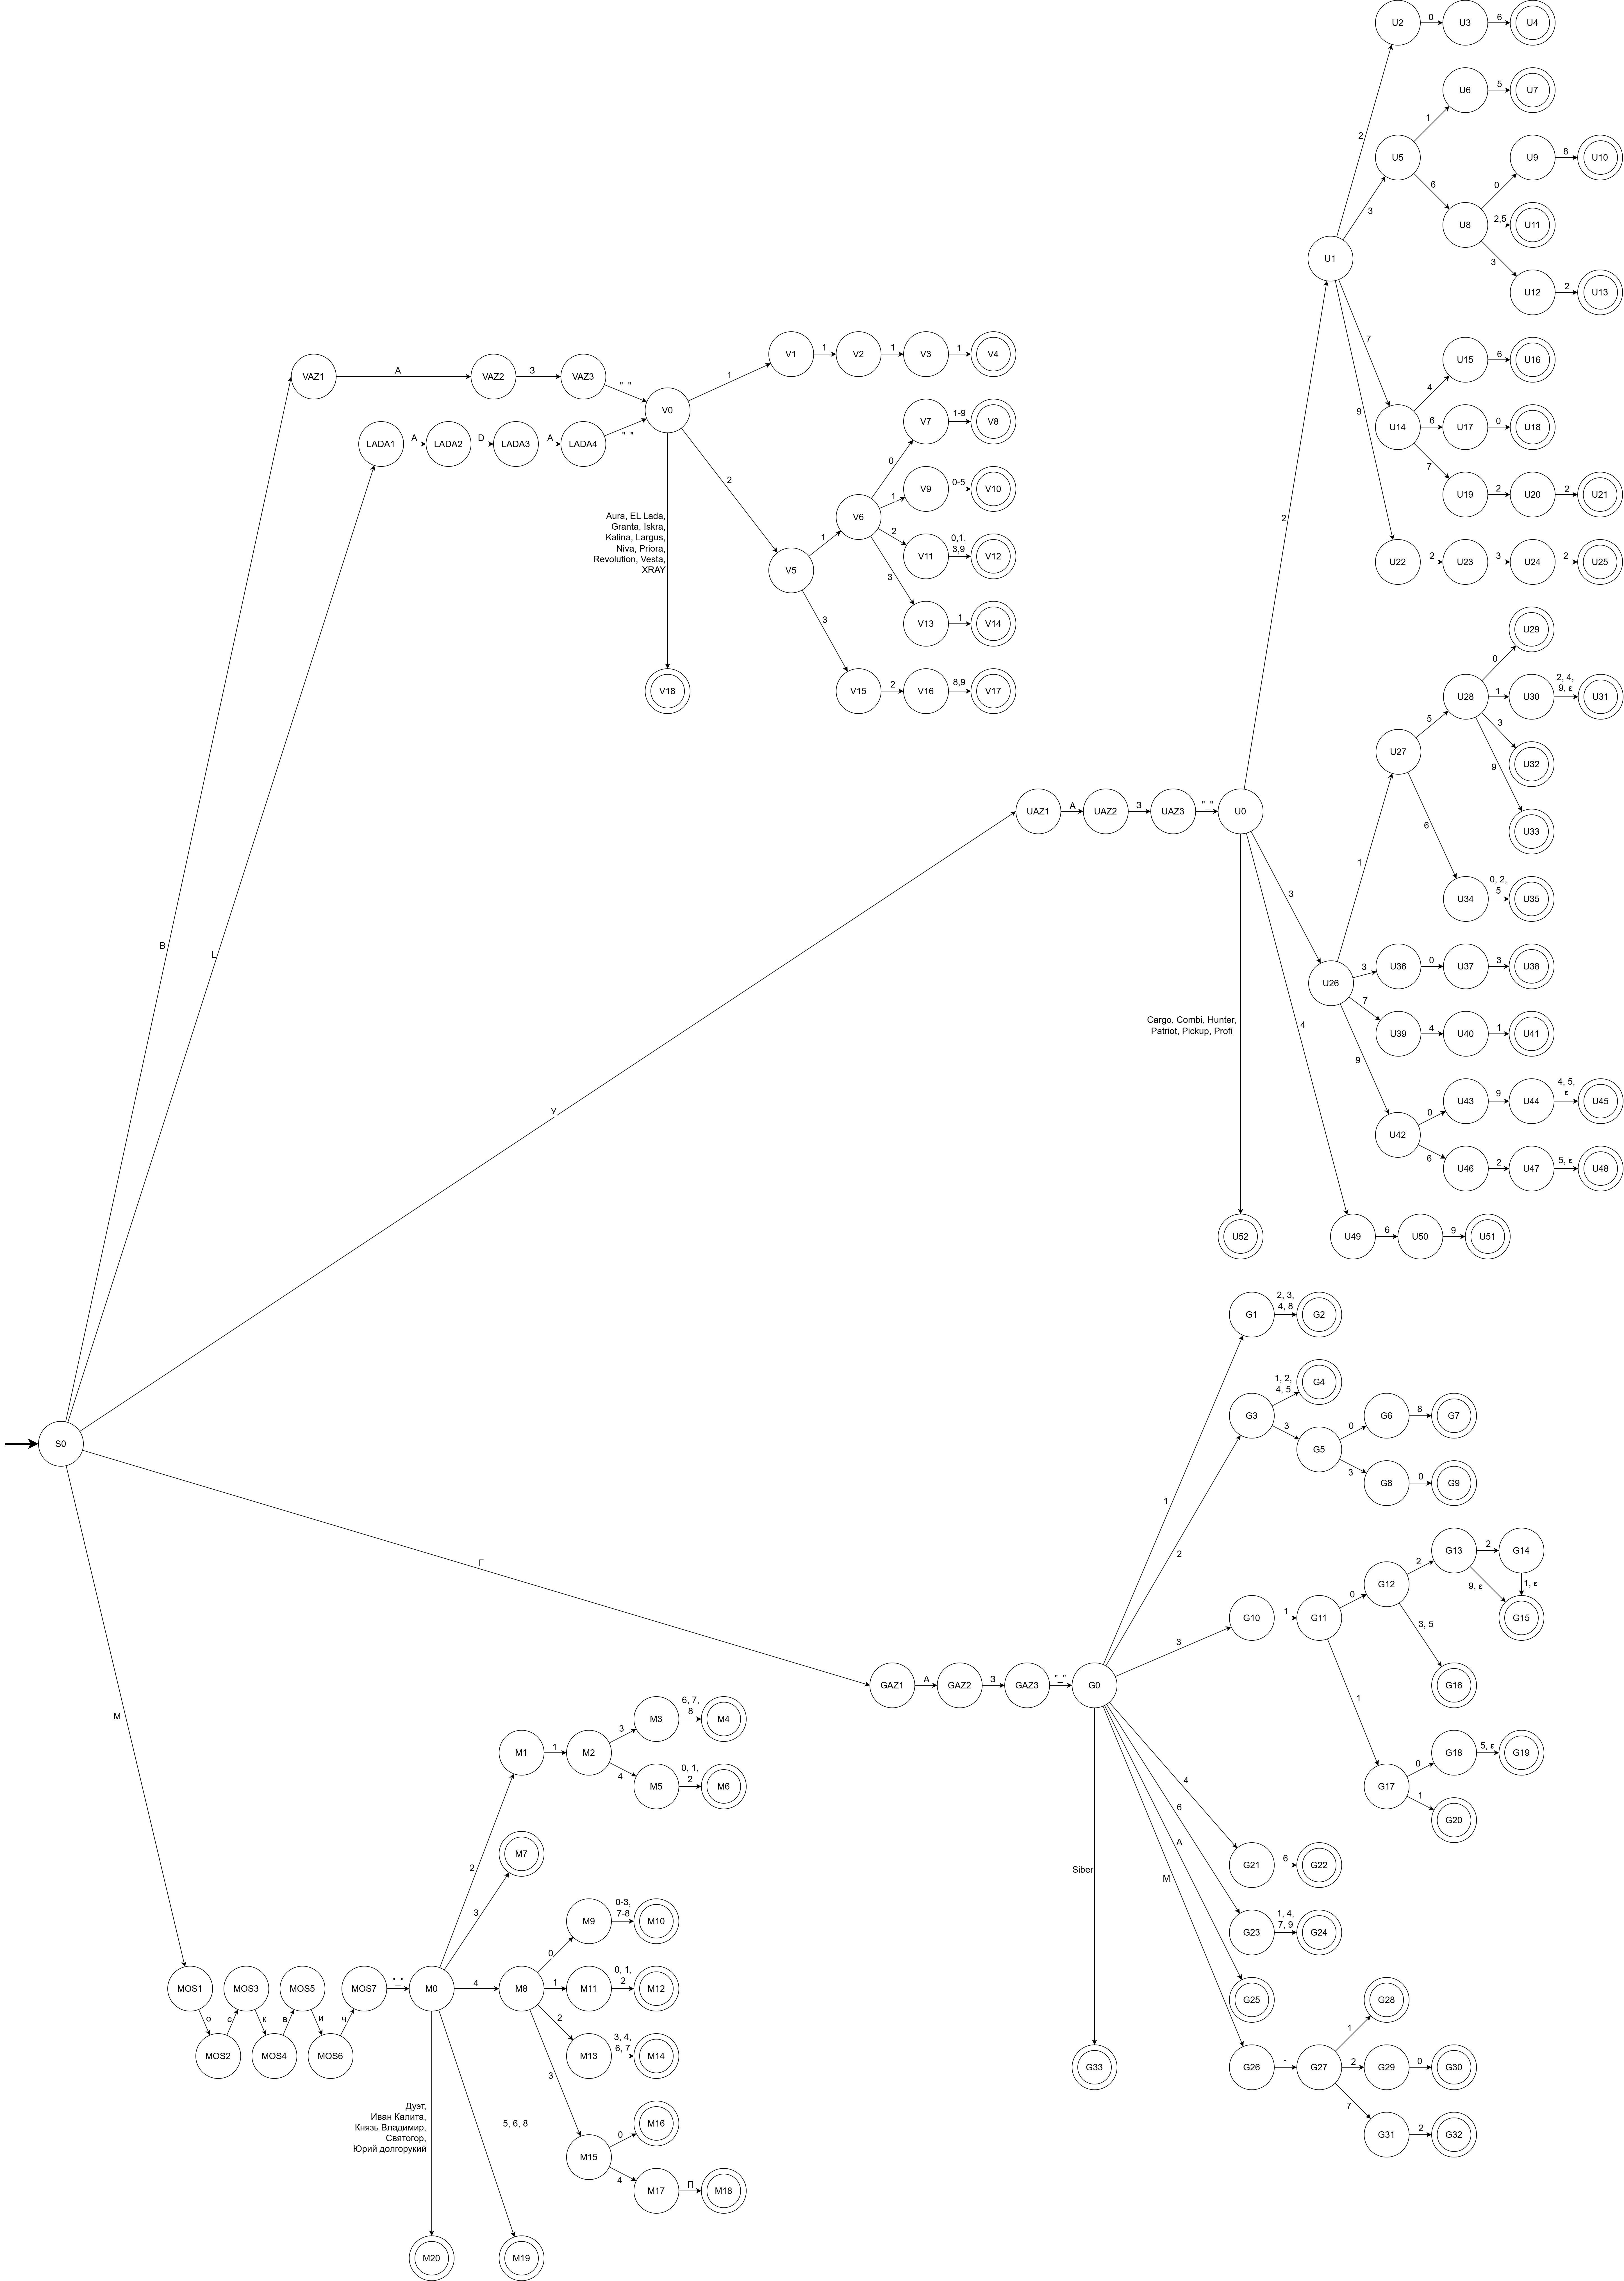
\includegraphics[width=1\linewidth]{NDKA_Lab2.jpg}
    \caption{\centeringНДКА для распознавания модели автомобиля}
\end{figure}

\subsection{Детерминированный конечный автомат}
Полученный детерминированный конечный автомат для рассматриваемого регулярного выражения представлен на рисунке 6.
\begin{figure}[H]
    \centering
    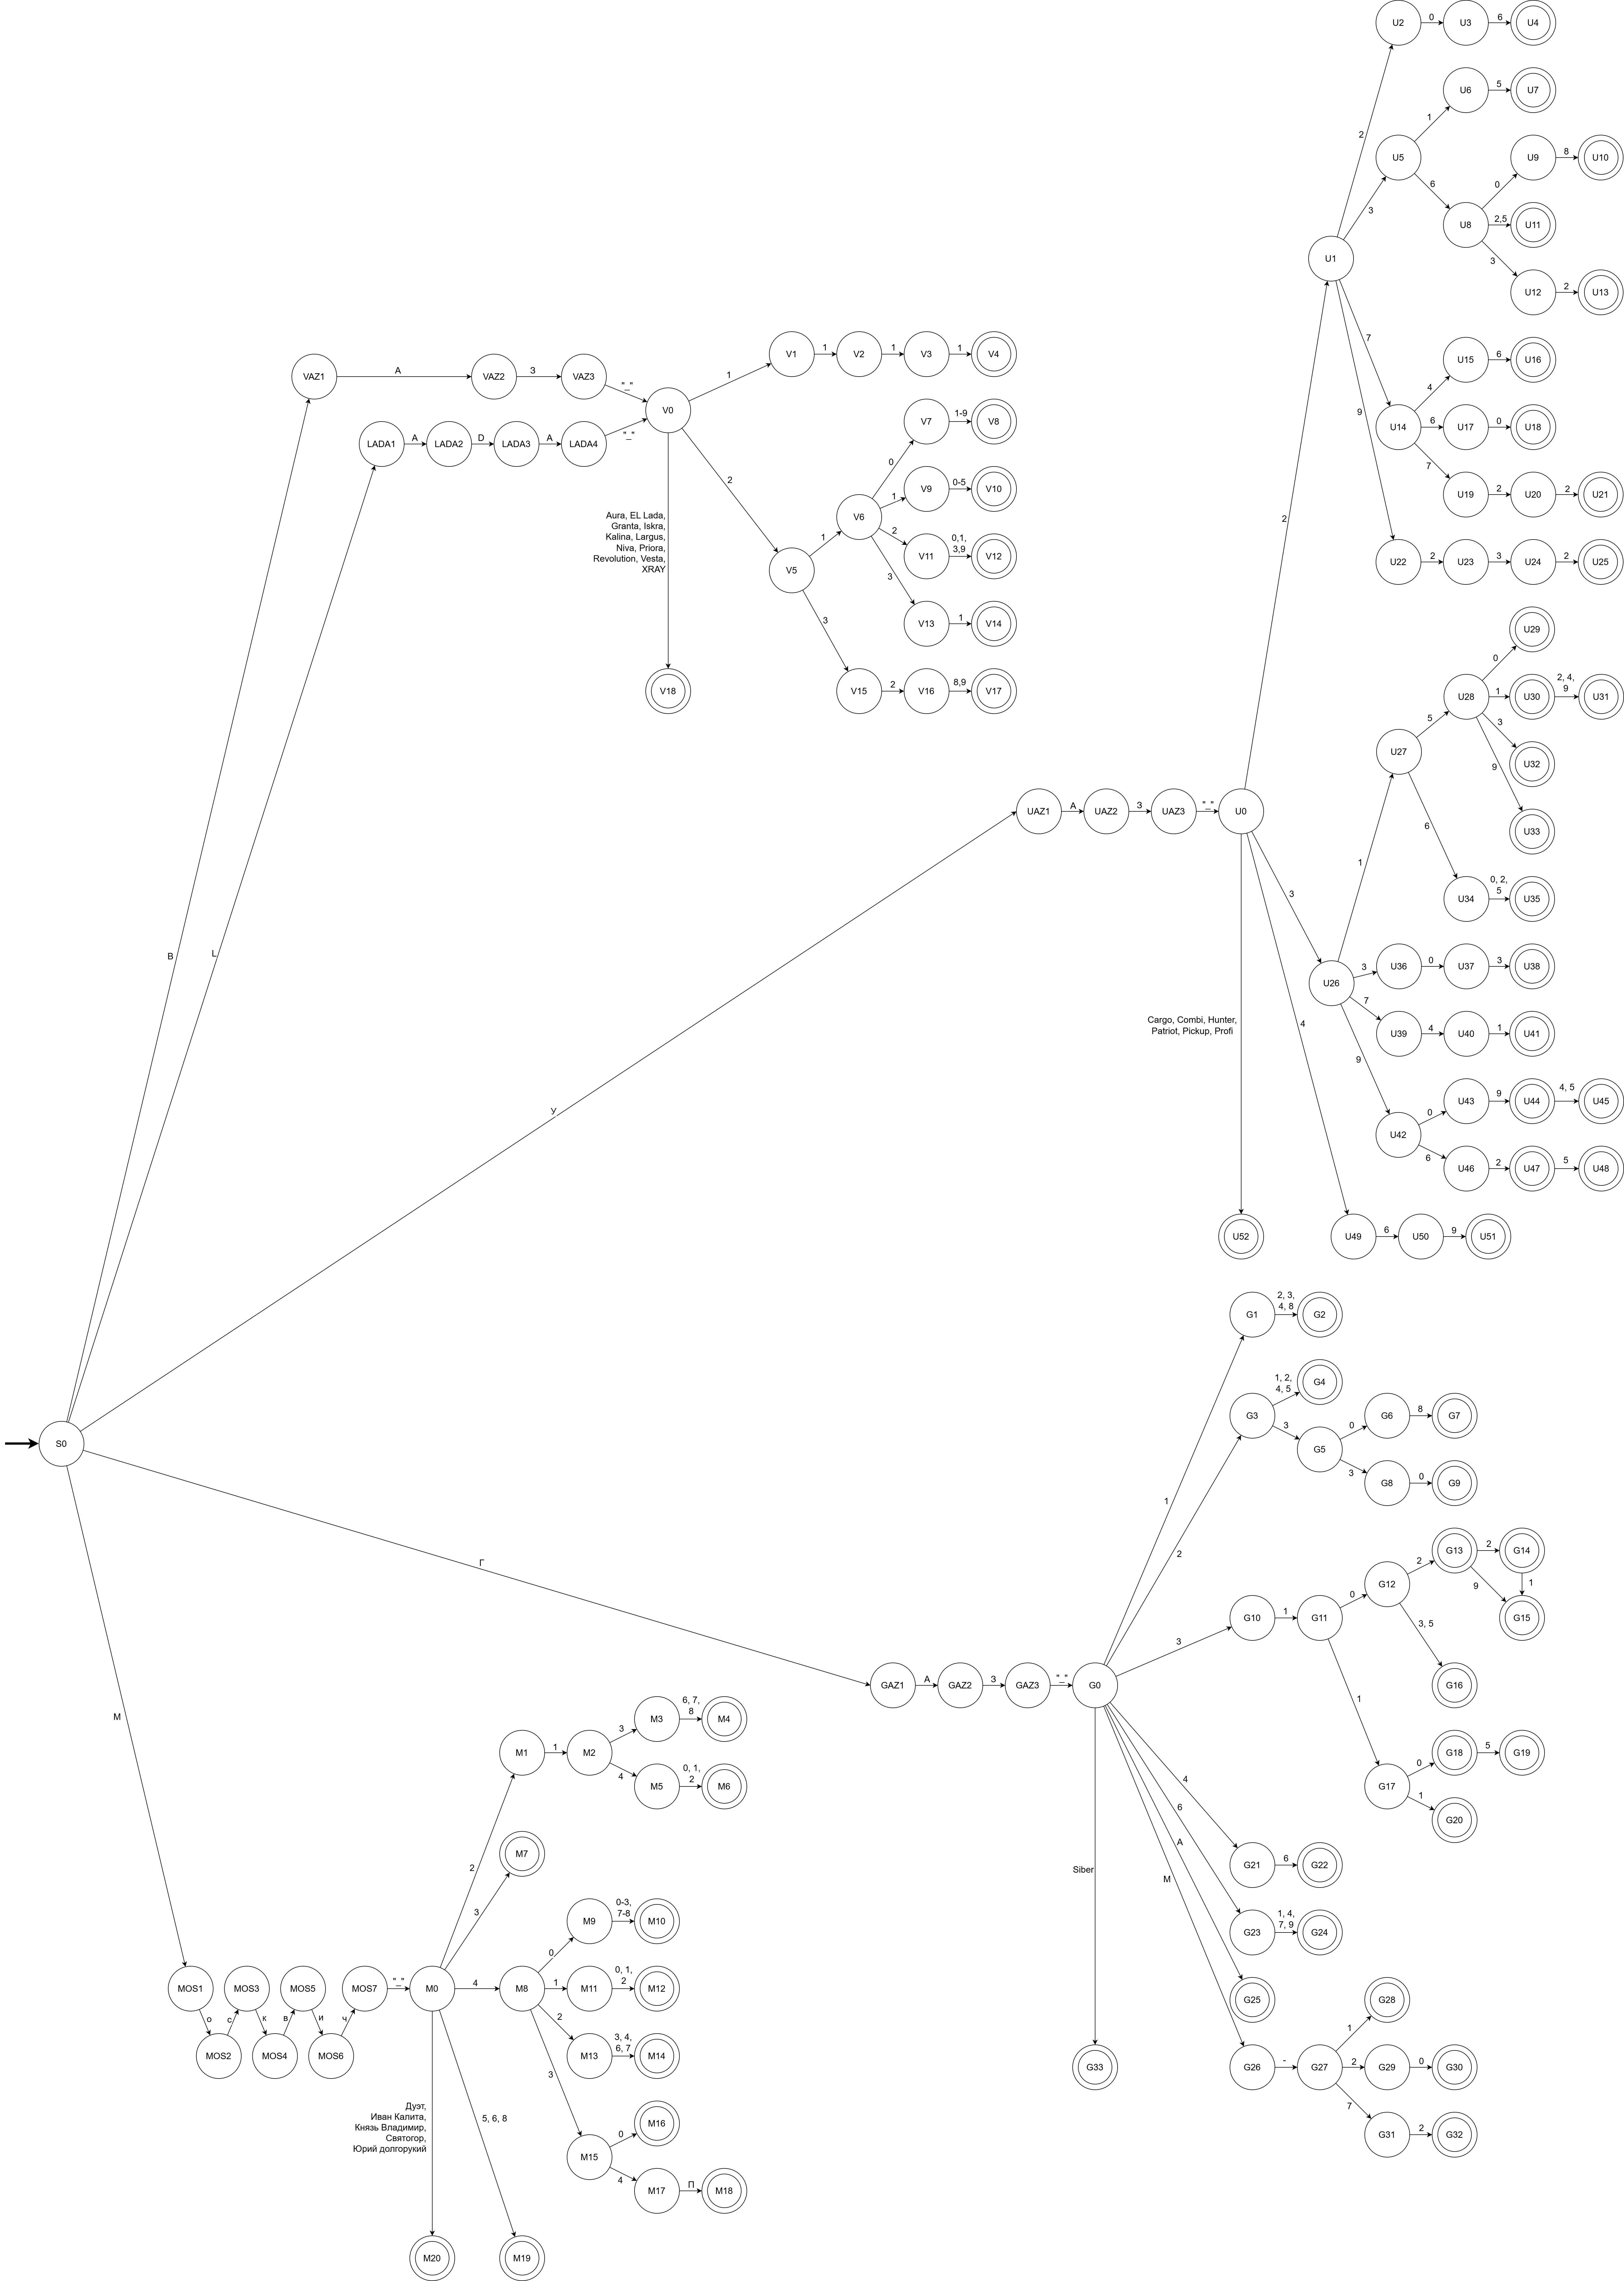
\includegraphics[width=0.9\linewidth]{DKA_Lab2.jpg}
    \caption{\centeringНДКА для распознавания модели автомобиля}
\end{figure}
В таблице 1 представлены переходы разработанного детерминированного конечного автомата.

\begin{longtable}{|c|c|c|}
\caption{Переходы детерминированного конечного автомата} \\
\hline
\textbf{Текущее состояние} & \textbf{Входящий символ} & \textbf{Следующее состояние} \\ \hline
\endfirsthead
\hline
\textbf{Текущее состояние} & \textbf{Входящий символ} & \textbf{Следующее состояние} \\ \hline
\endhead

\hline \multicolumn{3}{r}{{Продолжение на следующей странице}} \\
\endfoot

\hline
\endlastfoot

S0 & В & VAZ1 \\
S0 & L & LADA1 \\
S0 & У & UAZ1 \\
S0 & Г & GAZ1 \\
S0 & М & MOS1 \\
\hline

VAZ1 & А & VAZ2 \\
VAZ2 & З & VAZ3 \\
VAZ3 & << >> & V0 \\
LADA1 & A & LADA2 \\
LADA2 & D & LADA3 \\
LADA3 & A & LADA4 \\
LADA4 & << >> & V0 \\
V0 & \parbox{7cm}{Aura, Granta, Iskra, Kalina, Largus, Niva, Priora, Revolution, Vesta, XRAY} & V18 \\
V0 & 1 & V1 \\
V1 & 1 & V2 \\
V2 & 1 & V3 \\
V3 & 1 & V4 \\
V5 & 1 & V6 \\
V5 & 3 & V15 \\
V6 & 0 & V7 \\
V6 & 1 & V9 \\
V6 & 2 & V11 \\
V6 & 3 & V13 \\
V7 & 1-9 & V8 \\
V9 & 0-5 & V10 \\
V11 & 0, 1, 3, 9 & V12 \\
V13 & 1 & V14 \\
V15 & 2 & V16 \\
V16 & 8, 9 & V17 \\
\hline

UAZ1 & А & UAZ2 \\
UAZ2 & З & UAZ3 \\
UAZ3 & << >> & U0 \\
U0 & \parbox{7cm}{Cargo, Combi, Hunter, Patriot, Pickup, Profi} & U52 \\
U0 & 2 & U1 \\
U0 & 3 & U26 \\
U0 & 4 & U49 \\
U1 & 2 & U2 \\
U1 & 3 & U5 \\
U1 & 7 & U14 \\
U1 & 9 & U22 \\
U2 & 0 & U3 \\
U3 & 6 & U4 \\
U5 & 1 & U6 \\
U5 & 6 & U8 \\
U6 & 5 & U7 \\
U8 & 0 & U9 \\
U8 & 2, 5 & U11 \\
U8 & 3 & U12 \\
U9 & 8 & U10 \\
U12 & 2 & U13 \\
U14 & 5 & U15 \\
U14 & 6 & U17 \\
U14 & 7 & U19 \\
U15 & 6 & U16 \\
U17 & 0 & U18 \\
U19 & 2 & U20 \\
U20 & 2 & U21 \\
U22 & 2 & U23 \\
U23 & 3 & U24 \\
U24 & 2 & U25 \\
U26 & 1 & U27 \\
U26 & 3 & U36 \\
U26 & 7 & U39 \\
U26 & 9 & U42 \\
U27 & 5 & U28 \\
U27 & 6 & U34 \\
U28 & 0 & U29 \\
U28 & 1 & U30 \\
U28 & 3 & U32 \\
U28 & 9 & U33 \\
U30 & 2, 4, 9 & U31 \\
U36 & 0 & U37 \\
U37 & 3 & U38 \\
U39 & 4 & U40 \\
U40 & 1 & U41 \\
U42 & 0 & U43 \\
U42 & 6 & U46 \\
U43 & 9 & U44 \\
U44 & 4, 5 & U45 \\
U46 & 2 & U47 \\
U47 & 5 & U48 \\
U49 & 6 & U50 \\
U50 & 9 & U51 \\
\hline

GAZ1 & A & GAZ2 \\
GAZ2 & Z & GAZ3 \\
GAZ3 & << >> & G0 \\
G0 & Siber & G33 \\
G0 & 1 & G1 \\
G0 & 2 & G3 \\
G0 & 3 & G10 \\
G0 & 4 & G21 \\
G0 & 6 & G23 \\
G0 & А & G25 \\
G0 & М & G26 \\
G1 & 2, 3, 4, 8 & G2 \\
G3 & 1, 2, 4, 5 & G4 \\
G3 & 3 & G5 \\
G5 & 0 & G6 \\
G5 & 3 & G8 \\
G6 & 8 & G7 \\
G8 & 0 & G9 \\
G10 & 1 & G11 \\
G11 & 0 & G12 \\
G11 & 1 & G17 \\
G12 & 2 & G13 \\
G12 & 3, 5 & G16 \\
G13 & 2 & G14 \\
G13 & 9 & G15 \\
G14 & 1 & G15 \\
G17 & 0 & G18 \\
G18 & 5 & G19 \\
G21 & 6 & G22 \\
G23 & 1, 4, 7, 9 & G24 \\
G26 & - & G27 \\
G27 & 1 & G28 \\
G27 & 2 & G29 \\
G27 & 7 & G31 \\
G29 & 0 & G30 \\
G31 & 2 & G32 \\
\hline

% Ветвь Москвич (MOS)
MOS1 & о & MOS2 \\
MOS2 & с & MOS3 \\
MOS3 & к & MOS4 \\
MOS4 & в & MOS5 \\
MOS5 & и & MOS6 \\
MOS6 & ч & MOS7 \\
MOS7 & << >> & M0 \\
M0 & \parbox{7cm}{Дуэт, Иван Калита, Князь Владимир, Святогор, Юрий Долгорукий} & M20 \\
M0 & 2 & M1 \\
M0 & 3 & M7 \\
M0 & 4 & M8 \\
M0 & 5, 6, 8 & M19 \\
M1 & 1 & M2 \\
M2 & 3 & M3 \\
M2 & 4 & M5 \\
M3 & 6, 7, 8 & M4 \\
M5 & 0, 1, 2 & M6 \\
M8 & 0 & M9 \\
M8 & 1 & M11 \\
M8 & 2 & M13 \\
M8 & 3 & M15 \\
M9 & 0-3, 7, 8 & M10 \\
M11 & 0, 1, 2 & M12 \\
M13 & 3, 4, 6, 7 & M14 \\
M15 & 0 & M16 \\
M15 & 4 & M17 \\
M17 & П & M18 \\

\end{longtable}

\newpage
\section{Особенности реализации}
\subsection{Структуры данных}
Для данной лабораторной работы была разработан модуль, который позволяет:
\begin{itemize}
    \item Создавать детерминированные конечные автоматы с помощью:
    \begin{itemize}
        \item матрицы переходов и матрицы выходов;
        \item перечисления узлов с указанием их дочерних узлов;
        \item композиции уже существующих КА;
    \end{itemize}
    \item обрабатывать данные с помощью КА;
    \item генерировать случайные корректные данные подходящие под созданный КА.
\end{itemize}

Реализация конечного автомата выполнена с использованием шаблонов, что позволяет, используя один и тот же интерфейс, обрабатывать не только строки, но и любой перечисляемый тип данных, например вектора или массивы с любыми внутренними типами данных.

Также следует отметить, что выходами при переходах между состояниями КА являются выходы функций, а не константные значения, что позволяет при необходимости расширить создаваемый КА до КА с магазинной памятью. При создании КА также можно определить функцию-обработчик, которая будет обрабатывать выходы данных функций. С помощью изменения функции-обработчика можно реализовать логирование работы КА, определение символа на котором КА прекратил работу, подсчёт частоты появления символов во входных данных и т.д..

Для генерации случайных данных можно использовать уже созданный автомат. Программа позволяет автоматически найти для каждого перехода подходящие элементы из заданного алфавита с помощью одного обхода графа КА. Во время генерации данных можно указать вероятность с которой сгенерированные корректные данные будут случайным образом повреждены.


\subsubsection{Класс Action}
Данный класс реализует хранение действий при переходах между состояниями КА. Класс Action является обёрткой над обычной функцией с заданной сигнатурой. Использование данного класса позволяет совместно хранить и функции и Null значения, что полезно, если не все переходы в КА должны иметь выход. Код данного класса представлен на листинге 1.

\footnotesize{
\begin{lstlisting}[language=C++, caption = {Код класса Action}]
template<typename Signature>
class Action {
private:
    std::function<Signature> func;

public:
    Action() = default;
    Action(const Action& other) = default;

    Action(Action&& other) noexcept = default;

    template<typename F>
    requires (!std::is_same_v<std::decay_t<F>, Action<Signature>> && std::is_constructible_v<std::function<Signature>, F&&>)
    Action(F&& other);

    Action& operator=(Action&& other) noexcept;

    template<typename... Args>
    auto operator()(Args&&... args) const;

    explicit operator bool() const;

    void reset();
};
\end{lstlisting}
}
\small

Для данного класса был переопределён оператор вызова, который позволяет вызывая экземпляр данного класса выполнить функцию внутри него. Данный метод был объявлен шаблонным, чтобы сделать возможным вызов функций с разными сигнатурами.

Вход: аргументы для вызова внутренней функции.

Выход: выполненная внутренняя функция с заданными аргументами.

Код переопределения оператора вызова представлен на листинге 2.

\footnotesize{
\begin{lstlisting}[language=C++, caption = {Код переопределения оператора вызова}]
Action& Action::operator=(Action&& other) noexcept {
    if (this != &other) {
        func = std::move(other.func);
    }
    return *this;
}
\end{lstlisting}
}
\small

\subsubsection{Класс FSM}
Класс FSM реализует создание, хранение и использование конечных автоматов. Данный класс также объявленным шаблонным, что позволяет использовать один класс для работы с различными итерируемыми типами данных. В качестве шаблонов указывается тип входных данных, например строка или вектор чисел, и тип выходных данных при выполнении действий при переходах между узлами, например строка, символ, экземпляр какого-либо класса или void в случае если выходы при переходах не предусмотрены. Код данного класса представлен на листинге 3




\footnotesize{
\begin{lstlisting}[language=C++, caption = {Код класса FSM}]
template<typename Data, typename ActionOut>
    requires std::ranges::range<Data>
class FSM {
private:

    int currentState;

    using ElementType = std::ranges::range_value_t<Data>;
    using Condition = std::function<bool(ElementType)>;
    using ActionPtr = Action<ActionOut(ElementType)>*;
    using Harvester = std::function<void(ActionOut)>;

    ElementType element;

    std::deque<ElementType> dataProc;

    std::vector<ActionPtr> matrixActions;
    std::vector<Condition> matrixConditions;
    std::vector<int> matrixStates;

    std::vector<int> offsets;
    std::vector<int> finalStates;

    std::function<void(ActionOut)>outputsHarvester;

    std::vector<std::vector<ElementType>> elemsConditions;

    bool flagEnd = false;

    bool doStep();

    FSM(
        int stateCount,
        std::unordered_map<int, std::vector<std::tuple<int, Condition, ActionPtr>>> transitions,
        std::vector<int> finals,
        std::function<void(ActionOut)> harvester
    );

public:
    FSM() = default;

    FSM(
        std::vector<std::vector<Condition>> conditions,
        std::vector<std::vector<ActionPtr>> actions,
        std::vector<int> finals,
        std::function<void(ActionOut)> harvester = nullptr
    );

    using Transition = std::pair<int, std::pair<Condition, ActionPtr>>;
    using TransitionMap = std::unordered_map<int, std::vector<Transition>>;

    FSM(
        int stateCount,
        TransitionMap transitions,
        std::vector<int> finals,
        std::function<void(ActionOut)> harvester = nullptr
    );

    using TransitionNull = std::pair<int, Condition>;
    using TransitionMapNull = std::unordered_map<int, std::vector<TransitionNull>>;

    FSM(
        int stateCount,
        TransitionMapNull transitions,
        std::vector<int> finals,
        ActionPtr allAction = nullptr,
        std::function<void(ActionOut)> harvester = nullptr
    );


    FSMResult start(Data& data, int startState = 0, Data* alphabet = nullptr);

    std::deque<ElementType> getRemains();

    int getStateCount() const;

    std::vector<std::tuple<int, Condition, ActionPtr>> getTransitionsFrom(int state) const;

    bool isFinalState(int state) const;

    std::vector<int> getFinalStates() const;

    Harvester getHarvester() const;

	void genElemsOfConditions(Data* alphabet);
	Data genElem(std::mt19937& generator, Data* alphabet, float prop, int startState = 0);

    template<typename D, typename AO>
    friend FSM<D, AO> mergeFSM(
        const FSM<D, AO>& fsm1, int state1,
        const FSM<D, AO>& fsm2, int state2,
        std::function<void(AO)> harvester
    );
};
\end{lstlisting}
}
\small

\paragraph{Назначение полей класса\\[1em]}
\begin{itemize}
    \item currentState -- активный узел КА.
    \item element -- текущий обрабатываемый элемент из входных данных.
    \item dataProc -- входные данные, перезаписанные в двухстороннюю очередь, которая позволяет выполнять быстрое удаление значений из начала.
    \item matrixActions -- плоский вектор, хранящий матрицу выходов. Используется плоский вектор для обеспечения наилучшей кэш-лояльности.
    \item matrixConditions -- плоский вектор, хранящий матрицу переходов. В нём также используется плоский вектор.
    \item matrixStates -- вектор, содержащий номера узлов, входящих в данный конечный автомат.
    \item offsets -- вспомогательный вектор для определения в плоских векторах условий и действий, соответствующих определённому узлу.
    \item finalStates -- вектор, хранящий номера финальных состояний.
    \item outputsHarvester -- функция-обработчик выходов функций, использующихся при переходах. При любом заданном шаблоне возвращает void, так как использование данной функции предполагает использование захвата внешних переменных для хранения вычисляемых значений.
    \item elemsConditions -- двумерный вектор для хранения вычисленных допустимых элементов из входного алфавита для каждого узла.
\end{itemize}

Для класса FSM было реализовано три конструктора с разными входами.

Первый конструктор является наиболее сложным для ручного использования, так как требует записи матриц переходов и выходов. При использовании данного конструктора заданные матрицы просто копируются в поля данного экземпляра. Код данного конструктора представлен на листинге 4.

Вход: матрицы переходов и выходов, вектор финальных состояний, функцию-обработчик выходов.

Выход: созданный конечный автомат по заданным матрицам.

\footnotesize{
\begin{lstlisting}[language=C++, caption = {Код первого конструктора класса FSM}]
FSM(
    std::vector<std::vector<Condition>> conditions,
    std::vector<std::vector<ActionPtr>> actions,
    std::vector<int> finals,
    std::function<void(ActionOut)> harvester = nullptr
) : outputsHarvester(harvester)
{
    if (actions.size() == conditions.size()) {
        finalStates = finals;
        int stateCount = actions.size();
        offsets.reserve(stateCount + 1);
        offsets.push_back(0);

        for (int i = 0; i < stateCount; i++) {
            for (int j = 0; j < stateCount; j++) {
                if (conditions[i][j]) {
                    matrixActions.push_back(actions[i][j]);
                    matrixConditions.push_back(conditions[i][j]);
                    matrixStates.push_back(j);
                }
            }
            offsets.push_back(matrixActions.size());
        }
    }
}
\end{lstlisting}
}
\small

Второй и третий конструкторы являются более простыми способами создания конечных автоматов. При их использовании необходимо перечислить для каждого узла узлы КА, в которые возможен переход, условие перехода и действие при переходе. Третий конструктор отличается от второго тем, что не требует записи действия при переходе для каждого задаваемого перехода, а позволяет задать одно действие для всех переходов (например, функция, возвращающая полученный элемент). Коды данных конструкторов представлены на листинге 5.

Вход для второго конструктора: количество узлов в КА, словарь, содержащий перечисление узлов, условий перехода и действий при переходе для каждого узла КА, вектор финальных состояний и функция-обработчик выходов.

Вход для третьего конструктора: количество узлов в КА, словарь, содержащий перечисление узлов и условий перехода для каждого узла КА, вектор финальных состояний, действие при любом переходе и функция-обработчик выходов.

Выход: созданный конечный автомат с заданными узлами и переходами между ними.

\footnotesize{
\begin{lstlisting}[language=C++, caption = {Код второго и третьего конструкторов класса FSM}]
using Transition = std::pair<int, std::pair<Condition, ActionPtr>>;
using TransitionMap = std::unordered_map<int, std::vector<Transition>>;

FSM(
    int stateCount,
    TransitionMap transitions,
    std::vector<int> finals,
    std::function<void(ActionOut)> harvester = nullptr
) : outputsHarvester(harvester)
{
    finalStates = std::move(finals);
    offsets.resize(stateCount + 1);

    for (int state = 0; state < stateCount; ++state) {
        offsets[state] = static_cast<int>(matrixActions.size());
        
        auto it = transitions.find(state);
        if (it != transitions.end()) {
            for (const auto& [to, condAct] : it->second) {
                auto [condition, action] = condAct;
                if (condition) {
                    matrixActions.push_back(action);
                    matrixConditions.push_back(condition);
                    matrixStates.push_back(to);
                }
            }
        }
    }
    offsets[stateCount] = static_cast<int>(matrixActions.size());
}

using TransitionNull = std::pair<int, Condition>;
using TransitionMapNull = std::unordered_map<int, std::vector<TransitionNull>>;

FSM(
    int stateCount,
    TransitionMapNull transitions,
    std::vector<int> finals,
    ActionPtr allAction = nullptr,
    std::function<void(ActionOut)> harvester = nullptr
) : outputsHarvester(harvester)
{
    finalStates = std::move(finals);
    offsets.resize(stateCount + 1);

    for (int state = 0; state < stateCount; ++state) {
        offsets[state] = static_cast<int>(matrixActions.size());

        auto it = transitions.find(state);
        if (it != transitions.end()) {
            for (const auto& [to, cond] : it->second) {
                auto condition = cond;
                if (condition) {
                    matrixActions.push_back(allAction);
                    matrixConditions.push_back(condition);
                    matrixStates.push_back(to);
                }
            }
        }
    }
    offsets[stateCount] = static_cast<int>(matrixActions.size());
}
\end{lstlisting}
}
\small

Для перехода в следующий узел КА при заданных входных данных используется приватный метод doStep. Данный метод берёт следующий элемент из входных данных и проверяет возможность перехода в каждый следующий узел из текущего. Если существует подходящий переход, выполняется действие при переходе и вызывается функция обработчик выходов при переходах, а после меняется номер текущего состояния и возвращается значение true. Если переход не был найден, возвращается false. Выходные значения данного метода обрабатываются в методе start. Код метода doStep представлен на листинге 6.

Вход: текущее активное состояние в КА, входные данные, матрица переходов и действий при переходах, функция-обработчик выходов функций при переходах.

Выход: изменённое текущее активное состояние в КА и выполненное действие при переходе или изменённый флаг достижения финального состояния.

\footnotesize{
\begin{lstlisting}[language=C++, caption = {Код метода doStep}]
    bool doStep() {
        int condStart = offsets[currentState];
        int condEnd = offsets[currentState + 1];
        
        if (dataProc.size() > 0) {
            element = dataProc.front();
            dataProc.pop_front();
        }
        else {
            if (std::count(finalStates.begin(), finalStates.end(), currentState) > 0) {
                flagEnd = true;
                return false;
            }
        }

        for (int i = condStart; i < condEnd; i++) {
            if (matrixConditions[i](element)) {
                if (matrixActions[i]) {
                    ActionOut res = (*matrixActions[i])(element);
                    if (outputsHarvester) {
                        outputsHarvester(res);
                    }
                }
                currentState = matrixStates[i];

                return true;
            }
        }
        return false;
    };
\end{lstlisting}
}
\small

Для запуска обработки входных данных созданным КА необходимо использовать метод start. Данный метод перезаписывает входные данные в двухстороннюю очередь и последовательно выполняет переход к следующему состоянию с помощью метода doStep. Если больше нет доступных переходов или входные данные закончились, начинается обработка результатов, в течении которой определяется из-за чего завершилась работа КА: данные соответствуют (было достигнуто финальной состояние и входные данные закончились), был найден элемент не входящий в заданный алфавит или данные не соответствуют. Код данного метода можно увидеть на листинге 7.

Вход: входные данные, начальное состояние КА, алфавит входного языка.

Выход: выполненные действия при переходах, соответствующих входным данным и результат обработки данных.


\footnotesize{
\begin{lstlisting}[language=C++, caption = {Код метода start}]
FSMResult start(Data& data, int startState = 0, Data* alphabet = nullptr) {
    if (data.empty()) {
        return FSMResult::Mismatch;
    }
    if (startState < offsets.size() - 1) {
        dataProc.clear();
        for (const ElementType& element : data) {
            dataProc.push_back(element);
        }
        currentState = startState;
    }
    flagEnd = false;
    while (doStep()) { }
    if (flagEnd) {
        return FSMResult::Match;
    }
    if (alphabet) {
        for (ElementType alphElem : *alphabet) {
            if (alphElem == element) {
                return FSMResult::Mismatch;
            }
        }
        return FSMResult::OutOfAlphabet;
    }
    return FSMResult::Mismatch;
};
\end{lstlisting}
}
\small

Для хранения результата обработки входных данных был создан класс-перечисление FSMResult, который имеет три допустимых значения: подходит, не подходит, не из алфавита. Код определения данного перечисление представлен на листинге 8.
\footnotesize{
\begin{lstlisting}[language=C++, caption = {Код класса-перечисления FSMResult}]
enum class FSMResult {
    Match,
    Mismatch,
    OutOfAlphabet
};
\end{lstlisting}
}
\small

Для данного перечисления была создана функция resToStr, которая принимает его экземпляр и возвращает строку для вывода пользователю, соответствующую значению экземпляра. Код данной функции представлен на листинге 9.

Вход: результат обработки данных конечным автоматом.

Выход: строка, соответствующая полученному результату.

\footnotesize{
\begin{lstlisting}[language=C++, caption = {Код функции resToStr}]
wstring resToStr(FSMResult result) {
    switch (result) {
    case FSMResult::Match: return L"Строка соответствует";
    case FSMResult::Mismatch: return L"Строка не соответствует";
    case FSMResult::OutOfAlphabet:  return L"Используется символ не из алфавита";
    }
}
\end{lstlisting}
}
\small

Для построения композиции конечных автоматов была создана функция mergeFSM, которая <<склеивает>> заданные состояния двух КА. Данная функция создаёт новый экземпляр КА, в котором будет содержаться $n + m - 1$ состояний, где n и m -- количество узлов в первом и во втором КА соответственно. При этом следует отметить, что нумерация состояний изменяется -- состояния из первого КА остаются со своими номерами, а номер каждого состояния из второго КА сдвигается, так чтобы являться минимальным номером, не пересекающимся с номерами состояния из первого КА. Код функции mergeFSM представлен на листинге 10.

Вход: два КА и два номера состояний из первого и второго КА, которые необходимо <<склеить>> между собой.

Выход: новый конечный автомат, состоящий из узлов первого и второго КА так, что заданные состояния преобразованы в одно состояние.

\footnotesize{
\begin{lstlisting}[language=C++, caption = {Код функции mergeFSM}]
FSM<Data, ActionOut> mergeFSM(
    const FSM<Data, ActionOut>& fsm1, int state1,
    const FSM<Data, ActionOut>& fsm2, int state2,
    std::function<void(ActionOut)> harvester = nullptr
) {
    using Condition = typename FSM<Data, ActionOut>::Condition;
    using ActionPtr = typename FSM<Data, ActionOut>::ActionPtr;

    int n1 = fsm1.getStateCount();
    int n2 = fsm2.getStateCount();

    int totalStates = n1 + n2 - 1;

    std::unordered_map<int, std::vector<std::tuple<int, Condition, ActionPtr>>> transitions;


    for (int s = 0; s < n1; s++) {
        auto trans = fsm1.getTransitionsFrom(s);
        for (const auto& [to, cond, act] : trans) {
            transitions[s].emplace_back(to, cond, act);
        }
    }

	auto remapState = [&](int s) -> int {
		if (s == state2) {
			return state1;
		}
		else if (s < state2) {
			return s + n1;
		}
		else {
			return s + n1 - 1;
		}
		};

    for (int s = 0; s < n2; s++) {
        auto trans = fsm2.getTransitionsFrom(s);
        int fromRemapped = remapState(s);

        for (const auto& [to, cond, act] : trans) {
            int toRemapped = remapState(to);
            transitions[fromRemapped].emplace_back(toRemapped, cond, act);
        }
    }

    std::vector<int> finalStates;

    for (int fs : fsm1.getFinalStates()) {
        finalStates.push_back(fs);
    }

    for (int fs : fsm2.getFinalStates()) {
        int remapped = remapState(fs);
        if (std::find(finalStates.begin(), finalStates.end(), remapped) == finalStates.end()) {
            finalStates.push_back(remapped);
        }
    }
    return FSM<Data, ActionOut>(totalStates, std::move(transitions), std::move(finalStates), harvester);
}
\end{lstlisting}
}
\small

Для подготовки КА к генерации корректных входных данных используется метод genElemsOfConditions, которая производит полный обход графа данного КА. В ходе обхода для каждого узла вычисляются элементы из входного алфавита, которые позволяют совершить переход в один из следующих узлов. Найденные элементы записываются в соответствующую позицию двумерного вектора elemsConditions. Вызывать данный метод необходимо только в случае, если был изменён входной алфавит или предикаты переходов в узлы, иначе вызов метода никак не повлияет на дальнейшую генерацию корректных данных. Код данного метода представлен на листинге 11.

Вход: входной алфавит и матрица переходов КА.

Выход: вычисленные элементы входного алфавита, позволяющие выполнить переход, для каждого узла.

\footnotesize{
\begin{lstlisting}[language=C++, caption = {Код метода genElemsOfConditions}]
void genElemsOfConditions(Data* alphabet) {
	for (int i = 0; i < matrixConditions.size(); i++) {
        elemsConditions.push_back(std::vector<ElementType>());
		for (ElementType elem : *alphabet) {
            if (matrixConditions[i](elem)) {
                elemsConditions[i].push_back(elem);
            }
            
		}
	}
}
\end{lstlisting}
}
\small

После вызова метода genElemsOfConditions, можно начинать генерацию корректных входных данных. Для этого используется метод genElem, который случайным образом формирует путь по графу КА. При переходе в новый узел случайным образом выбирается элемент, позволяющий выполнить переход, полученный элемент добавляется к результирующей переменной и производится переход в следующее состояние, соответствующее выбранному элементу. При вызове данного метода можно указать вероятность специальной <<порчи>> корректных данных -- если в случайное число оказывается меньше заданной вероятности, то случайный элемент из результирующей переменной заменяется на случайный элемент из входного алфавита. Код данного метода представлен на листинге 12.

Вход: генератор случайных чисел, входной алфавит, вероятность <<порчи данных>> и начальное состояние из КА при генерации.

Выход: случайным образом сформированные входные данные, которые могут оказаться испорчены с заданной вероятностью.

\footnotesize{
\begin{lstlisting}[language=C++, caption = {Код метода genElem}]
Data genElem(std::mt19937& generator, Data* alphabet, float prop, int startState = 0) {
    if (elemsConditions.empty()) {
        return Data();
    }
    currentState = startState;

    Data res;
	
    while (true) {
		int condStart = offsets[currentState];
		int condEnd = offsets[currentState + 1];
        if (condStart == condEnd) {
            break;
        }
        if (std::count(finalStates.begin(), finalStates.end(), currentState) > 0) {
            std::uniform_int_distribution<> dist0(0, 1);
            if (dist0(generator) == 1) {
                break;
            }
        }

        std::uniform_int_distribution<> dist1(condStart, condEnd - 1);
        int i = dist1(generator);
        std::uniform_int_distribution<> dist2(0, elemsConditions[i].size() - 1);
        int j = dist2(generator);

        res.push_back(elemsConditions[i][j]);
        currentState = matrixStates[i];
    }

	std::uniform_real_distribution<double> dist(0.0, 1.0);
	if (dist(generator) <= prop) {
        std::uniform_int_distribution<> dist1(0, res.size() - 1);
        std::uniform_int_distribution<> dist2(0, alphabet->size());
        res[dist1(generator)] = (*alphabet)[dist2(generator)];
	}
    
    return res;
};
\end{lstlisting}
}
\small

Также для упрощения создания конечных автоматов, обрабатывающих строки, была создана функция fsmFromWstr. Эта функция создаёт конечный автомат, который принимает только заданную строку. Для создания КА создаётся матрица действий при переходах, содержащая заданное действие для каждого перехода, и диагональная матрица переходов со сдвигом значений вправо. Код данной функции представлен на листинге 13.

Вход: строка, которую должен принимать КА, действие выполняемое при переходах и функция-обработчик выходов функций.

Выход: экземпляр конечного автомата, который принимает заданную строку.

\footnotesize{
\begin{lstlisting}[language=C++, caption = {Код функции fsmFromWstr}]
FSM<std::wstring, wchar_t> fsmFromWstr(std::wstring data, Action<wchar_t(wchar_t)>* allAction = nullptr, std::function<void(wchar_t)> harvester = nullptr) {
    int n = data.size();
    std::vector<std::vector<std::function<bool(wchar_t)>>> conditions(n + 1, std::vector<std::function<bool(wchar_t)>>(n + 1, nullptr));
    std::vector<std::vector<Action<wchar_t(wchar_t)>*>> actions(n + 1, std::vector<Action<wchar_t(wchar_t)>*>(n + 1, allAction));
    std::vector<int> finals({n});

    for (int i = 0; i < n; i++) {
        conditions[i][i+1] = [value = data[i]](wchar_t c) {return c == value; };
    }

    FSM<std::wstring, wchar_t> result(conditions, actions, finals, harvester);

    return result;
}
\end{lstlisting}
}
\small

\subsection{Функция обработки пользовательского ввода}

Для взаимодействия пользователя с программой была реализована функция userIO, которая предлагает пользователю варианты действий и выполняет действие исходя из ввода пользователя.

Вход: экземпляр КА с входными данными типа wstring, а выходными данными типа wchar\_t, и строки, формирующиеся с помощью пользовательского ввода.

Выход: вывод меню пользователю и выполнение действий выбранных пользователем.

Данная функция представляет следующие меню:
\begin{enumerate}
    \item \textbf{Главное меню}: пользователю предлагается выполнить одно из следующих действий:
    \begin{itemize}
        \item ввести строку;
        \item сгенерировать строки;
        \item сменить реализацию программы (КА или регулярное выражение);
        \item выйти из программы.
    \end{itemize}
    \item \textbf{Ввод строки}. У пользователя запрашивается ввод строки требующей проверки на соответствие регулярному выражению. После правильного ввода, программа обрабатывает полученную строку и выводит информацию о результате обработки.
    \item \textbf{Генерация строк}. У пользователя запрашивается требуемое количество строк и вероятность <<порчи>> корректной строки. После правильного ввода программа генерирует заданной количество строк, обрабатывает их и выводит сводку о результатах обработки (количество соответствующих, не соответствующих и имеющих символы не из алфавита). 
    
    При необходимости программа может вывести все обработанные строки с цветовым выделением принятой и отброшенной частей строки.
\end{enumerate}

Код данной функции представлен на листинге 14.

\footnotesize{
\begin{lstlisting}[language=C++, caption = {Код функции userIO}]
void userIO(FSM<wstring, wchar_t> fsm) {
    while (true) {
        wcout << L"\nВыберите дейстие:\n\t[1] Ввести строку\n\t[2] Сгенерировать строки\n\t[3] Реализация (" << realization(useRegex) << L")\n\t[e] Выход" << endl;
        wstring input;
        getline(wcin, input);

        vector<wstring> vecStr;


        if (input == L"1") {
            wcout << L"Введите строку: ";
            wstring data;
            getline(wcin, data);
            vecStr.push_back(data);
        }
        else if (input == L"2") {
            int count = 0;
            float prop = 0;
            while (true) {
                wcout << L"Введите кол-во строк: ";
                string data;

                getline(cin, data);
                auto [ptr, ec] = std::from_chars(data.data(), data.data() + data.size(), count);

                if (ec == std::errc{}) {
                    if (count < 1 || count > 5000) {
                        wcout << L"\nВведённое число выходит за дапазон [1, 5000]. Повторите попытку." << endl;
                        continue;
                    }
                    break;
                }
                else if (ec == std::errc::invalid_argument) {
                    wcout << L"Неверный ввод. Повторите попытку." << endl;
                    continue;
                }
                else {
                    wcout << L"Введённое число выходит за дапазон [1, 5000]. Повторите попытку." << endl;
                    continue;
                }
            }

            while (true) {
                wcout << L"Введите вероятность случайной замены символа в строке: ";
                string data;

                getline(cin, data);
                auto [ptr, ec] = std::from_chars(data.data(), data.data() + data.size(), prop);

                if (ec == std::errc{} and ptr == data.data() + data.size()) {
                    if (prop < 0 || prop > 1) {
                        wcout << L"Введённое число выходит за дапазон [0, 1]. Повторите попытку." << endl;
                        continue;
                    }
                    break;
                }
                else if (ec == std::errc::invalid_argument) {
                    wcout << L"Неверный ввод. Повторите попытку." << endl;
                    continue;
                }
                else {
                    wcout << L"Введённое число выходит за дапазон [0, 1]. Повторите попытку." << endl;
                    continue;
                }
            }
            for (int i = 0; i < count; i++) {
                vecStr.push_back(fsm.genElem(gen, &alphabet, prop, 33));
            }
            wcout << L"Сгенерировано " << count << L" строк." << endl;
        }
        else if (input == L"3") {
            useRegex = !useRegex;
            continue;
        }
        else if (input == L"e") {
            wcout << L"Выход из программы" << endl;
            break;
        }
        else {
            wcout << L"Неверный ввод. Повторите попытку." << endl;
            continue;
        }

        FSMResult res;

        wstring result;

        int countSucc = 0;
        int countFail = 0;
        
        auto start = std::chrono::steady_clock::now();
        for (wstring s : vecStr) {
            if (useRegex) {
                if (areAllCharsIn(s, alphabet)) {
                    if (regex_match(s, re)) {
                        res = FSMResult::Match;
                        countSucc++;
                        result += L"\"\033[48;2;0;70;0m" + s + L"\033[40m\": " + resToStr(res) + L"\n";
                    }
                    else {
                        res = FSMResult::Mismatch;
                        countFail++;
                        result += L"\033[48;2;200;0;0m" + s + L"\033[40m\": " + resToStr(res) + L"\n";
                    }
                }
                else {
                    res = FSMResult::OutOfAlphabet;
                    result += L"\033[48;2;200;0;0m" + s + L"\033[40m\": " + resToStr(res) + L"\n";
                }
            }
            else {
                failureStr = s;
                successStr.clear();
                res = fsm.start(s, 33, &alphabet);

                if (res == FSMResult::Match) {
                    countSucc++;
                }
                else if (res == FSMResult::Mismatch) {
                    countFail++;
                }
                result += L"\"\033[48;2;0;70;0m" + successStr + L"\033[48;2;200;0;0m" + failureStr + L"\033[40m\": " + resToStr(res) + L"\n";
            }
        }
        auto end = std::chrono::steady_clock::now();
        std::chrono::duration<double, std::milli> time = end - start;

        wcout << L"Строки обработаны за " << time.count() << L" мс.\n";
        wcout << countSucc << L" строк соответствует" << endl;
        wcout << countFail << L" строк не соответствует" << endl;
        wcout << vecStr.size() - countSucc - countFail << L" строк имеют символы не из алфавита" << endl;
        while (true) {
            wcout << L"\nВывести результаты обработки?\n\t[1] Да\n\t[2] Нет" << endl;
            getline(wcin, input);
            if (input == L"1") {
                wcout << L"Обработанные строки:" << endl;
                wcout << result << endl;
                break;
            }
            else if (input == L"2") {
                break;
            }
            else {
                wcout << L"Неверный ввод. Повторите попытку." << endl;
                continue;
            }
        }
        vecStr.clear();
    }
}
\end{lstlisting}
}
\small
\subsection{Создание конечного автомата соответствующего заданному регулярному выражению}
Для создание конечного автомата, который сможет определять корректность введённых моделей автомобилей марок ВАЗ, УАЗ, ГАЗ, Москвич было создано 4 КА, каждый из которых реализует обработку моделей определённой марки. Каждый КА был создан с помощью перечисления узлов и следующих за ними узлов с их условиями переходов. 

Для всех переходов в КА был задан один выход -- функция baseAction, которая реализует базовое выходное действие -- передачу полученного символа дальше в функцию-обработчик выходов. 

Код данной функции представлен на листинге 15.

Вход: символ из входных данных.

Выход: символ, полученный во входе.

\footnotesize{
\begin{lstlisting}[language=C++, caption = {Код функции baseAction}]
Action<wchar_t(wchar_t)> baseAction([](wchar_t c) { return c; });
\end{lstlisting}
}
\small

Далее последовательно к созданным КА была применена функция mergeFSM, для создания композиции КА. При создании итоговой композиции КА была задана функция обработчик, которая разделяет входную строку на две части: принятая часть и отброшенная часть для формирования удобного вывода с использованием цветового выделения частей. 

Код данной функции представлен на листинге 16.

Вход: символ из входной строки.

Выход: изменённые принятая и отброшенная части входной строки.

\footnotesize{
\begin{lstlisting}[language=C++, caption = {Код класса harv\_log}]
function<void(wchar_t)> harv_log([](wchar_t c) {
    successStr.push_back(c);
    failureStr.erase(0, 1);
    });
\end{lstlisting}
}
\small

Код задания состояний и переходов всех созданных конечных автоматов можно увидеть в приложении А.

\newpage
\section{Результаты работы программы}

После запуска программы пользователю выводится главное меню (рисунок 7).
\begin{figure}[H]
    \centering
    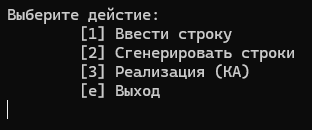
\includegraphics[width=0.5\linewidth]{main_menu.png}
    \caption{\centeringГлавное меню}
\end{figure}

После выбора действия <<Ввести строку>> и ввода строки, которую необходимо обработать, программа выводит сводку об обработке полученной строки и далее можно вывести более подробную информацию о введённой строке (рисунок 8). 

\begin{figure}[H]
    \centering
    \begin{subfigure}[b]{0.45\textwidth}
            \centering
            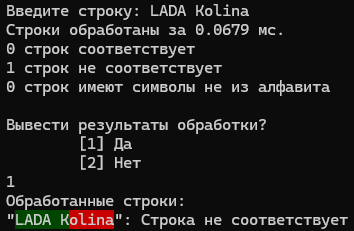
\includegraphics[width=1\linewidth]{image.png}
            \caption{\centeringНесоответствующая строка}
    \end{subfigure}
    \hfill % Распорка для равномерного распределения
    \begin{subfigure}[b]{0.45\textwidth}
            \centering
            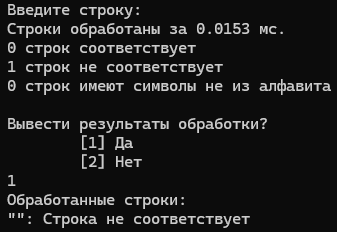
\includegraphics[width=1\linewidth]{image0.png}
            \caption{\centeringПустая строк}
    \end{subfigure}
    \caption{\centeringВывод информации об обработанной строке}
    \label{fig:both}
\end{figure}

Также пользователь может в главном меню выбрать пункт <<Сгенерировать строки>>, после чего программа потребует от него ввода количества строк и вероятности случайной замены символа в корректной строке. Для количества строк определено ограничение в 5000, так как вывод в консоль большего количества строк будет очень долгим, а для вероятности заданы границы от 0 до 1 включительно. На рисунке 9 представлен ввод количества строк и вероятности случайной замены символа.
\begin{figure}[H]
    \centering
    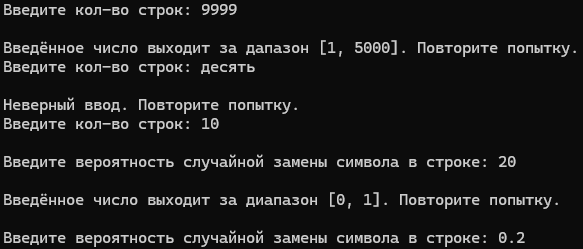
\includegraphics[width=0.6\linewidth]{image1.png}
    \caption{\centeringВвод количества строк и вероятности замены символа}
\end{figure}

После успешного ввода количества строк и вероятности, пользователю выводится краткая сводка об обработанных строках и по желанию пользователя выводится детальный вывод каждой строки (рисунок 10). В выводе подробной информации зелёным цветом выделяется часть строки, которую КА смог принять, а красным -- не принятая часть.
\begin{figure}[H]
    \centering
    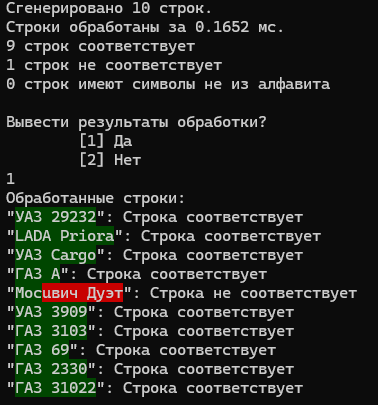
\includegraphics[width=0.5\linewidth]{image2.png}
    \caption{\centeringВывод сводки и подробной информации об обработанных строках}
\end{figure}

Также пользователь может изменить реализацию программу выбрав вместо конечного автомата использование регулярного выражения с помощью модуля regex. При использовании реализации через КА в среднем строки обрабатываются в два раза быстрее, чем при использовании регулярного выражения. На рисунке 11 представлено сравнение скорости обработки одной и той же строки с использованием разных реализаций. 

Следует отметить, что при использовании реализации через regex вывод подробной информации об обработанных строках упрощается, так как regex не поддерживает нахождение индекса символа, с которого началось несоответствии заданному регулярному выражению.

\begin{figure}[H]
    \centering
    \begin{subfigure}[b]{0.45\textwidth}
            \centering
            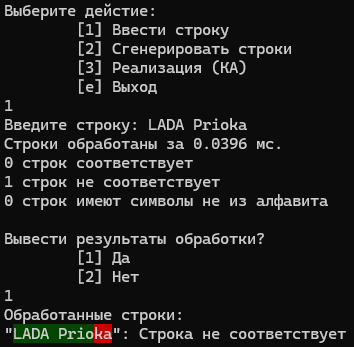
\includegraphics[width=1\linewidth]{image3.png}
            \caption{\centeringС использованием КА}
    \end{subfigure}
    \hfill % Распорка для равномерного распределения
    \begin{subfigure}[b]{0.45\textwidth}
            \centering
            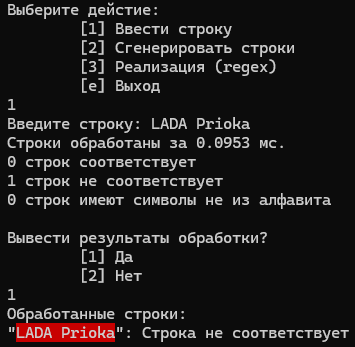
\includegraphics[width=1\linewidth]{image4.png}
            \caption{\centeringС использованием regex}
    \end{subfigure}
    \caption{\centeringСравнение скорости обработки строки с помощью разных реализаций}
    \label{fig:both}
\end{figure}

\newpage
\section*{Заключение}
\addcontentsline{toc}{section}{Заключение}

В ходе выполнения данной лабораторной работы было создано регулярное выражение, соответствующее моделям автомобилей марок ВАЗ, УАЗ, ГАЗ и Москвич. На основе полученного регулярного выражения были созданы недетерминированный КА и детерминированный КА, который состоит из 295 состояний. 

Далее был разработан модуль для создания КА и работы с ними и с помощью него было реализовано программное представление составленного детерминированного конечного автомата.

Реализованная программа предоставляет пользователю следующие функции:
\begin{itemize}
    \item обработка введённой пользователем строки;
    \item генерация до 5000 строк с задаваемой пропорцией несоответствующих строк и последующая обработка сгенерированных строк;
    \item смена реализации программы (КА или регулярное выражение);
\end{itemize}

\paragraph{Достоинства реализации}
\begin{itemize}
    \item Разработанный модуль позволяет реализовывать конечные автоматы, обрабатывающие не только строки, но и любые итерируемые данные. Также с помощью модуля можно создавать автоматы с магазинной памятью, что позволяет использовать данный модуль при создании распознавателей контекстно-свободных языков.
    \item Для генерации корректных строк, используется алгоритм, который автоматически для каждого перехода находит подходящие символы заданного входного алфавита. Асимптотическая сложность данного алгоритма составляет $O(q \cdot |\Sigma|)$, где q -- количество переходов, а $|\Sigma|$ -- количество символов во входном алфавите. Данный алгоритм запускается только один раз, после чего генерация строки происходит без лишних вычислений.
    \item Пользователю предоставляется возможность выбора реализации программы (использование модуля regex или использование КА).
    \item Реализована цветовое выделение принятой и не принятой частей входной строки.
    \item Разработанный КА в среднем работает более чем в два раза быстрее, чем соответствующее ему регулярное выражение в модуле regex.
\end{itemize}
\paragraph{Недостатки реализации}
\begin{itemize}
    \item Распределение вероятности генерации корректных строк неравномерное -- наибольшая вероятность генерации у корректных строк, состоящих из наименьшего количества символов.
\end{itemize}
\paragraph{Масштабирование}
\begin{itemize}
    \item Добавить графический интерфейс для создания КА из созданного модуля или реализовать создание КА из файлов формата <<.drawio>>, содержащих графическое описание КА.
    \item Реализовать преобразование регулярного выражения в КА из созданного модуля.
\end{itemize}

\newpage
\addcontentsline{toc}{section}{Список использованной литературы}
\begin{thebibliography}{}
    \bibitem{litlink1} Секция <<Телематика>>.— Текст: электронный // tema.spbstu: [сайт].— URL: https://tema.spbstu.ru/mathem/ (дата обращения: 29.03.2026).
    \bibitem{litlink2} Вирт, Н. Построение компиляторов / Н. Вирт. – М.: ДМК Пресс, 2010. – 190 с.

    \bibitem{litlink3} Ахо, А. В. Компиляторы: принципы, технологии и инструментарий [2-е изд.] / А. В. Ахо, М. С. Лам, Р. Сети, Дж. Д. Ульман ; Пер. с англ. — М. : ООО «И.Д. Вильямс», 2018. — 1184 с.
\end{thebibliography}






\newpage
\section*{Приложение A. Исходный код создания конечных автоматов}
\addcontentsline{toc}{section}{Приложение A. Исходный код создания конечных автоматов}
\footnotesize{
\begin{lstlisting}[language=C++]
wstring alphabet = L" -0123456789ACDEGHIKLMNPRSVXYabcdefgiklmnoprstuvАВГДЗИКМПСУЮавгдзийклмнорстучьэя";

Action<wchar_t(wchar_t)> baseAction([](wchar_t c) { return c; });


bool (*is0)(wchar_t) = [](wchar_t c) { return c == L'0'; };
bool (*is1)(wchar_t) = [](wchar_t c) { return c == L'1'; };
bool (*is2)(wchar_t) = [](wchar_t c) { return c == L'2'; };
bool (*is3)(wchar_t) = [](wchar_t c) { return c == L'3'; };
bool (*is4)(wchar_t) = [](wchar_t c) { return c == L'4'; };
bool (*is5)(wchar_t) = [](wchar_t c) { return c == L'5'; };
bool (*is6)(wchar_t) = [](wchar_t c) { return c == L'6'; };
bool (*is7)(wchar_t) = [](wchar_t c) { return c == L'7'; };
bool (*is8)(wchar_t) = [](wchar_t c) { return c == L'8'; };
bool (*is9)(wchar_t) = [](wchar_t c) { return c == L'9'; };


FSM<wstring, wchar_t>::TransitionMapNull tG;
tG[0] = {
    {1, is1},
    {3, is2},
    {10, is3},
    {21, is4},
    {23, is6},
    {25, [](wchar_t c) { return c == L'А'; }},
    {26, [](wchar_t c) { return c == L'М'; }}
};
tG[1] = {
    {2, [](wchar_t c) { return c == L'2' || c == L'3' || c == L'4' || c == L'8'; }},
};
tG[2] = {};
tG[3] = {
    {4, [](wchar_t c) { return c == L'1' || c == L'2' || c == L'4' || c == L'5'; }},
    {5, is3}
};
tG[4] = {};
tG[5] = {
    {6, is0},
    {8, is3}
};
tG[6] = {
    {7, is8}
};
tG[7] = {};
tG[8] = {
    {9, is0}
};
tG[9] = {};
tG[10] = {
    {11, is1}
};
tG[11] = {
    {12, is0},
    {17, is1}
};
tG[12] = {
    {13, is2},
    {16, [](wchar_t c) { return c == L'3' || c == L'5'; }}
};
tG[13] = {
    {14, is2},
    {15, is9}
};
tG[14] = {
    {15, is1}
};
tG[15] = {};
tG[16] = {};
tG[17] = {
    {18, is0},
    {20, is1}
};
tG[18] = {
    {19, is5}
};
tG[19] = {};
tG[20] = {};
tG[21] = {
    {22, is6}
};
tG[22] = {};
tG[23] = {
    {24, [](wchar_t c) { return c == L'1' || c == L'4' || c == L'7' || c == L'9'; }}
};
tG[24] = {};
tG[25] = {};
tG[26] = {
    {27, [](wchar_t c) { return c == L'-'; }}
};
tG[27] = {
    {28, is1},
    {29, is2},
    {31, is7}
};
tG[28] = {};
tG[29] = {
    {30, is0}
};
tG[30] = {};
tG[31] = {
    {32, is2}
};
tG[32] = {};
tG[33] = { // start
    {34, [](wchar_t c) { return c == L'Г'; }}
};
tG[34] = {
    {35, [](wchar_t c) { return c == L'А'; }}
};
tG[35] = {
    {36, [](wchar_t c) { return c == L'З'; }}
};
tG[36] = {
    {0, [](wchar_t c) { return c == L' '; }}
};
FSM<wstring, wchar_t> fsmG(
    37,
    tG,
    { 2, 4, 7, 9, 13, 14, 15, 16, 18, 19, 20, 22, 24, 25, 28, 30, 32 },
    &baseAction,
    nullptr
);
vector<wstring> strsG = { L"Siber" };
for (wstring s : strsG) {
    fsmG = mergeFSM(fsmG, 0, fsmFromWstr(s, &baseAction), 0);
}


FSM<wstring, wchar_t>::TransitionMapNull tU;
tU[0] = {
    {1, is2},
    {26, is3},
    {49, is4},
    {56, [](wchar_t c) {return c == L'C'; }},
    {57, [](wchar_t c) {return c == L'P'; }}
};
tU[1] = {
    {2, is2},
    {5, is3},
    {14, is7},
    {22, is9}
};
tU[2] = {
    {3, is0}
};
tU[3] = {
    {4, is6}
};
tU[4] = {};
tU[5] = {
    {6, is1},
    {8, is6}
};
tU[6] = {
    {7, is5}
};
tU[7] = {};
tU[8] = {
    {9, is0},
    {11, [](wchar_t c) {return c == L'2' || c == L'5'; }},
    {12, is3}
};
tU[9] = {
    {10, is8}
};
tU[10] = {};
tU[11] = {};
tU[12] = {
    {13, is2}
};
tU[13] = {};
tU[14] = {
    {15, is4},
    {17, is6},
    {19, is7}
};
tU[15] = {
    {16, is6}
};
tU[16] = {};
tU[17] = {
    {18, is0}
};
tU[18] = {};
tU[19] = {
    {20, is2}
};
tU[20] = {
    {21, is2}
};
tU[21] = {};
tU[22] = {
    {23, is2}
};
tU[23] = {
    {24, is3}
};
tU[24] = {
    {25, is2}
};
tU[25] = {};
tU[26] = {
    {27, is1},
    {36, is3},
    {39, is7},
    {42, is9}
};
tU[27] = {
    {28, is5},
    {34, is6}
};
tU[28] = {
    {29, is0},
    {30, is1},
    {32, is3},
    {33, is9}
};
tU[29] = {};
tU[30] = {
    {31, [](wchar_t c) {return c == L'2' || c == L'4' || c == L'9'; }}
};
tU[31] = {};
tU[32] = {};
tU[33] = {};
tU[34] = {
    {35, [](wchar_t c) {return c == L'0' || c == L'2' || c == L'5'; }}
};
tU[35] = {};
tU[36] = {
    {37, is0}
};
tU[37] = {
    {38, is3}
};
tU[38] = {};
tU[39] = {
    {40, is4}
};
tU[40] = {
    {41, is1}
};
tU[41] = {};
tU[42] = {
    {43, is0},
    {46, is6}
};
tU[43] = {
    {44, is9}
};
tU[44] = {
    {45, [](wchar_t c) {return c == L'4' || c == L'5'; }}
};
tU[45] = {};
tU[46] = {
    {47, is2}
};
tU[47] = {
    {48, is5}
};
tU[48] = {};
tU[49] = {
    {50, is6}
};
tU[50] = {
    {51, is9}
};
tU[51] = {};
tU[52] = { // start
    {53, [](wchar_t c) {return c == L'У'; }}
};
tU[53] = {
    {54, [](wchar_t c) {return c == L'А'; }}
};
tU[54] = {
    {55, [](wchar_t c) {return c == L'З'; }}
};
tU[55] = {
    {0, [](wchar_t c) {return c == L' '; }}
};
tU[56] = {};
tU[57] = {};
FSM<wstring, wchar_t> fsmU(
    58,
    tU,
    { 4, 7, 10, 11, 13, 16, 18, 21, 25, 29, 30, 31, 32, 33, 35, 38, 41, 44, 45, 47, 48, 51 },
    & baseAction,
    nullptr
);
fsmU = mergeFSM(fsmU, 0, fsmFromWstr(L"Hunter", &baseAction), 0);
vector<wstring> strsU1 = { L"argo", L"ombi" };
for (wstring s : strsU1) {
    fsmU = mergeFSM(fsmU, 56, fsmFromWstr(s, &baseAction), 0);
}
vector<wstring> strsU2 = { L"atriot", L"ickup", L"rofi" };
for (wstring s : strsU2) {
    fsmU = mergeFSM(fsmU, 57, fsmFromWstr(s, &baseAction), 0);
}


FSM<wstring, wchar_t>::TransitionMapNull tM;
tM[0] = {
    {1, is2},
    {7, is3},
    {8, is4},
    {19, [](wchar_t c) {return c == L'5' || c == L'6' || c == L'8'; }}
};
tM[1] = {
    {2, is1}
};
tM[2] = {
    {3, is3},
    {5, is4}
};
tM[3] = {
    {4, [](wchar_t c) {return c == L'6' || c == L'7' || c == L'8'; }}
};
tM[4] = {};
tM[5] = {
    {6, [](wchar_t c) {return c == L'0' || c == L'1' || c == L'2'; }}
};
tM[6] = {};
tM[7] = {};
tM[8] = {
    {9, is0},
    {11, is1},
    {13, is2},
    {15, is3}
};
tM[9] = {
    {10, [](wchar_t c) {return L'0' <= c && c <= L'3' || c == L'7' || c == L'8'; }}
};
tM[10] = {};
tM[11] = {
    {12, [](wchar_t c) {return L'0' <= c && c <= L'2'; }}
};
tM[12] = {};
tM[13] = {
    {14, [](wchar_t c) {return c == L'3' || c == L'4' || c == L'6' || c == L'7'; }}
};
tM[14] = {};
tM[15] = {
    {16, is0},
    {17, is4}
};
tM[16] = {};
tM[17] = {
    {18, [](wchar_t c) {return c == L'П'; }}
};
tM[18] = {};
tM[19] = {};
tM[20] = { // start
    {21, [](wchar_t c) {return c == L'М'; }}
};
tM[21] = {
    {22, [](wchar_t c) {return c == L'о'; }}
};
tM[22] = {
    {23, [](wchar_t c) {return c == L'с'; }}
};
tM[23] = {
    {24, [](wchar_t c) {return c == L'к'; }}
};
tM[24] = {
    {25, [](wchar_t c) {return c == L'в'; }}
};
tM[25] = {
    {26, [](wchar_t c) {return c == L'и'; }}
};
tM[26] = {
    {27, [](wchar_t c) {return c == L'ч'; }}
};
tM[27] = {
    {0, [](wchar_t c) {return c == L' '; }}
};
FSM<wstring, wchar_t> fsmM(
    28,
    tM,
    { 4, 6, 7, 10, 12, 14, 16, 18, 19 },
    & baseAction,
    nullptr
);
vector<wstring> strsM = { L"Дуэт", L"Иван Калита", L"Князь Владимир", L"Святогор", L"Юрий Долгорукий" };
for (wstring s : strsM) {
    fsmM = mergeFSM(fsmM, 0, fsmFromWstr(s, &baseAction), 0);
}


FSM<wstring, wchar_t>::TransitionMapNull tV;
tV[0] = {
    {1, is1},
    {5, is2}
};
tV[1] = {
    {2, is1}
};
tV[2] = {
    {3, is1}
};
tV[3] = {
    {4, is1}
};
tV[4] = {};
tV[5] = {
    {6, is1},
    {15, is3}
};
tV[6] = {
    {7, is0},
    {9, is1},
    {11, is2},
    {13, is3}
};
tV[7] = {
    {8, [](wchar_t c) {return L'0' <= c && c <= L'9'; }}
};
tV[8] = {};
tV[9] = {
    {10, [](wchar_t c) { return L'0' <= c && c <= L'5'; }}
};
tV[10] = {};
tV[11] = {
    {12, [](wchar_t c) {return c == L'0' || c == L'1' || c == L'3' || c == L'9'; }}
};
tV[12] = {};
tV[13] = {
    {14, is1}
};
tV[14] = {};
tV[15] = {
    {16, is2}
};
tV[16] = {
    {17, [](wchar_t c) {return c == L'8' || c == L'9'; }}
};
tV[17] = {};
tV[18] = { // start
    {19, [](wchar_t c) {return c == L'В'; }},
    {22, [](wchar_t c) {return c == L'L'; }}
};
tV[19] = {
    {20, [](wchar_t c) {return c == L'А'; }}
};
tV[20] = {
    {21, [](wchar_t c) {return c == L'З'; }}
};
tV[21] = {
    {0, [](wchar_t c) {return c == L' '; }}
};
tV[22] = {
    {23, [](wchar_t c) {return c == L'A'; }}
};
tV[23] = {
    {24, [](wchar_t c) {return c == L'D'; }}
};
tV[24] = {
    {25, [](wchar_t c) {return c == L'A'; }}
};
tV[25] = {
    {0, [](wchar_t c) {return c == L' '; }}
};
FSM<wstring, wchar_t> fsmV(
    26,
    tV,
    { 4, 8, 10, 12, 14, 17 },
    & baseAction,
    nullptr
);
vector<wstring> strsV = { L"Aura", L"EL Lada", L"Granta", L"Iskra", L"Kalina", L"Largus", L"Niva", L"Priora", L"Revolution", L"Vesta", L"XRAY", };
for (wstring s : strsV) {
    fsmV = mergeFSM(fsmV, 0, fsmFromWstr(s, &baseAction), 0);
}


function<void(wchar_t)> harv_log([](wchar_t c) {
    successStr.push_back(c);
    failureStr.erase(0, 1);
    });

FSM<wstring, wchar_t> fsmAll = mergeFSM(
    mergeFSM(fsmG, 33, fsmU, 52), 
    33, 
    mergeFSM(fsmM, 20, fsmV, 18), 
    20,
    harv_log
);

fsmAll.genElemsOfConditions(&alphabet);

userIO(fsmAll);
\end{lstlisting}
}
\small
\end{document}